\chapter{Faster Discovery of Faster System Configurations with Spectral Learning}
\label{chapter:WHAT}
\noindent\textit{This chapter originally appeared as Nair, V., Menzies, T., Siegmund, N., \& Apel, S. (2017). Faster discovery of faster system configurations with spectral learning. Automated Software Engineering, 1-31. }





\section{Abstract}
Despite the huge spread and economical importance of configurable software systems, there is  unsatisfactory support in utilizing the full potential of these systems with respect to finding performance-optimal configurations.
Prior work on predicting the performance of software configurations suffered from either (a)~requiring far too many sample configurations or (b)~large variances in their predictions.
Both these problems can be avoided using the \what spectral learner.  
{\what}'s innovation is  
the use of the spectrum (eigenvalues) of the distance matrix
between the configurations of a configurable software system, to perform dimensionality reduction. Within that
reduced configuration space, many closely associated configurations can be studied
by executing only a few sample configurations. For the subject systems studied
here, a few dozen samples yield accurate and stable predictors---less than 10\,\% prediction error, with a standard deviation of less than 2\,\%.  
When compared to the state of the art, our approach (a)~requires 
2 to 10 times fewer samples to achieve similar prediction accuracies,
and (b)~its predictions are  more stable (i.e., have lower standard
deviation). 
%unclear: (i.e., much mean errors and standard deviations on the errors, refer to Figure 9-11)
Furthermore, we demonstrate that predictive models generated by
\what can be used by optimizers to discover system configurations that closely approach the optimal performance.
%\keywords{Performance Prediction \and Spectral Learning \and Decision Trees \and Search-Based Software Engineering \and Sampling.}

\section{Introduction}
 
%==Are these comments?== 
%Are feature/variability models too abstract for concrete reasoning?
%Or is it possible to use these models to predict specific properties 
%of programs generated from them? 

Most software systems today are configurable. Despite the undeniable benefits
of configurability, 
large configuration spaces challenge developers, maintainers, and users. In the face of hundreds of configuration options, it is difficult to keep track of the effects of individual configuration options and their mutual interactions. So, predicting the performance of individual system configurations or determining the optimal configuration is often more guess work than engineering. In their recent paper, Xu et al.\ documented the  difficulties developers face
with understanding  the configuration spaces of their systems~\cite{xu2015hey}. As a result, developers tend to ignore over $5/6$ths of the configuration options, which leaves considerable optimization potential untapped and induces major economic cost~\cite{xu2015hey}.

Addressing the challenge of performance prediction and optimization in the face of large configuration spaces, researchers have developed a number of approaches that rely on sampling and machine learning~\cite{siegmund2012predicting,guo2013variability,sarkar2015cost}.
While gaining some ground, state-of-the-art approaches face two problems: 
(a)~they require far too many sample configurations for learning or (b)~they are prone to large variances in their predictions. For example, prior work on predicting performance scores using regression-trees had to compile and execute hundreds to thousands of specific system configurations~\cite{guo2013variability}. 
% Other studies that tried to make far fewer execution samples resulted in predictors that were considerably inaccurate in their performance predictions.\todo[inline]{Which do you mean?}
A more balanced approach by Siegmund et al.\ is able to learn predictors for  configurable systems~\cite{siegmund2012predicting} with low mean errors, but with large variances of prediction accuracy  (e.g.\ in half of the results, the performance predictions for the Apache Web server were up to 50\,\% wrong). 
%My(Norbert) comment on this: you can't just take the worst heuristic here when the paper was about improving over this worst case...
 %\footnote{The predictions of \cite{siegmund2012predicting} had $\mu=19\%$ errors with $\sigma = 19.5\%$.}
  %that half they time, they could be up to 50\% incorrect\footnote{
 %The range  $\mu \pm 1.5*\sigma$  includes the
 %25th to 75th percentile range of a normal distribution   
%For the \cite{siegmund2012predicting} errors, that range is  0 to 49\%.}. 
% >> Where do you have this data from? Does not match with the paper.
% Vivek: You take the fault rate and standard deviation of the method which uses **almost** same  number of measurements. 
Guo et al.~\cite{guo2013variability} also proposed an incremental method to build a predictor model, which uses incremental random samples with steps equal to the number of configuration options (features) of the system. This approach also
suffered from  unstable predictions (e.g., predictions had a mean error of up to 22\,\%, with a standard deviation of up 46\,\%). Finally, Sarkar et al.~\cite{sarkar2015cost} proposed a proj\-ective-learning approach (using fewer measurements than Guo at al.\ and Siegmund et al.) to quickly compute  the number of sample configurations for learning a stable predictor. However, as we will discuss, after making that prediction, the total number of samples required for learning the predictor is comparatively high (up to hundreds of samples).

The problems of large sample sets and large variances in prediction can be avoided using the \what spectral learner, which is our main contribution.  
{\what}'s innovation is  the use of the spectrum (eigenvalues) of the distance matrix
between the configurations of a configurable system, to perform dimensionality reduction. Within that
reduced configuration space, many closely associated configurations can be studied
by measuring only a few samples.
In a number of experiments, we compared \what against the state-of-the-art approaches of Siegmund et al.~\cite{siegmund2012predicting}, Guo et al.~\cite{guo2013variability}, and Sarkar et al. \cite{sarkar2015cost} by means of six real-world configurable systems: Berkeley DB,  the Apache Web server, SQLite, the LLVM compiler, and the x264 video encoder.
We found that \what performs as well or better than prior approaches,
while  requiring far fewer samples (just a few dozen).
This is significant and most surprising, since some of the systems explored here have up to millions of possible configurations. 

Overall, we make the following contributions:
\begin{itemize}
\item We present a novel sampling and learning approach for predicting the performance of software configurations in the face of large configuration spaces. The approach is based on a
{\em spectral
learner} that uses an approximation to the first principal component of the configuration space to recursively cluster it, relying only on a few points as representatives of each cluster.
\item We demonstrate the practicality and generality of our approach by conducting experiments on six real-world configurable software systems (see Figure ~\ref{fig:systems}). The results show that our approach is more accurate (lower mean error) and more stable (lower standard deviation) than state-of-the-art approaches.
\item We report on a comparative analysis of our approach and three state-of-the-art approaches, demonstrating that our approach outperforms previous approaches in terms of sample size and prediction stability. A key finding is the utility of the principal component of a configuration space to  find informative samples from a large configuration space.
\end{itemize}
%More generally, this paper illustrates the value of spectral learning for software-engineering data sets. We recommend spectral learning for any analytics
%tasks with many options described by sets of attributes
%that might be noisy or redundant. For further details on why we make this recommendation, see Section~\ref{sect:sample}.

%The rest of the paper is organized as follows. Section 2 defines the terms used in the paper. Section 3 describes the background of the problem we are trying to tackle along with the data sets used in the experiments. Section 4 further explores the research question and finds association among them. Section 5 describes the experiment setup etc. Section 6 discusses the results and Section 7 the related work. This paper concludes after mentioning the threats to validity.
 
\section{Background \& Related Work}  
\label{sect:addit}

A configurable software system has a set $X$ of Boolean configuration options,\footnote{In this paper, we concentrate on Boolean options, as they make up the majority of all options; see Siegmund et al., for how to incorporate numeric options~\cite{SGA+15}.} also referred to as features or independent variables in our setting.
We denote the number of features of system $S$ as $n$. The configuration space of $S$ can be represented by a Boolean space ${Z}_{2}^{n}$, which is denoted by $F$. All valid configurations of $S$ belong to a set $V$, 
which is represented by vectors $\vec{C_i}$ (with $1\leq i\leq \left\vert{V}\right\vert$) in ${Z}_{2}^{n}$. Each element of a configuration represents a feature, which can either be \emph{True} or \emph{False}, based on whether the feature is selected or not. 
% We denote the number of features in the system as $n$. All the features of a system can be represents a boolean/binary space (${Z}_{2}^{n}$)--- $F$, where $n$ is the number of features of the system. Every software system has a set of valid configurations ($V$) which is represented as a vector $\vec{C} \in {Z}_{2}^{n}$, where ${Z}_{2}^{n}$
% % http://math.stackexchange.com/questions/892094/notation-for-show-that-a-variable-is-binary
% is Boolean $n$-space i.e. each feature of a configurations is assigned $\mathit{True}$ and $\mathit{False}$ otherwise, based on whether the feature was selected or not.  
Each valid instance of a vector (i.e., a configuration) has a corresponding performance score associated to it. 

The literature offers two approaches to performance prediction of software configurations: a {\em maximal sampling} and a {\em minimal sampling} approach: 
With {\em maximal sampling}, we compile all  possible configurations and record the associated performance scores. 
Maximal sampling  can be impractically slow. For example, the performance data used in this paper required  26 days of CPU time for measuring (and much longer, if we also count the time required for compiling the code prior to execution). 
 Other researchers have commented that,  in 
 real world scenarios, the cost of acquiring the optimal configuration is overly expensive and time consuming \cite{weiss2008maximizing}.
 
 If collecting performance scores of all configurations is impractical,  {\em minimal sampling} 
 can be used to intelligently select and execute just enough configurations (i.e., samples) to build a
 predictive model.
 For example, Zhang et al.~\cite{zhang2015performance} approximate the
configuration space as a Fourier series, after which they can derive an expression showing how many configurations must be studied
 to build predictive models with a given error. While a theoretically satisfying result, that approach still needs thousands to hundreds of thousands of executions of sample
 configurations.  

Another set of approaches are the four "additive" {\em minimal sampling} methods of Siegmund et al.~\cite{siegmund2012predicting}.
Their first method, called feature-wise sampling ({\em FW}), is their basic method.
To explain {\em FW}, we note that, from a configurable software system, it is theoretically possible to enumerate many or all of the valid configurations\footnote{Though, in practice, this can be very difficult. For example, in models like the Linux Kernel such an enumeration is practically impossible ~\cite{sayyad13b}.}. 
Since each configuration ($\vec{C_i}$) is a vector of $n$ Booleans, it  is possible to use this information to isolate examples of how much each feature individually contributes to the total run time:
\begin{enumerate}
\item Find a pair of  configurations $\vec{C_i}$ and $\vec{C}_2$, where $\vec{C}_2$ uses exactly the same features as $\vec{C_i}$, plus one  extra feature $f_i$.
\item Set the run time $\Pi(f_i)$ for feature $f_i$ to be the difference in the performance scores between $\vec{C_2}$ and $\vec{C_i}$.
\item The run time  for a new configuration  $\vec{C}_i$ (with $1\leq i\leq \left\vert{V}\right\vert$) that has not been sampled before is then the sum of the run time of its features, as determined before:
\begin{equation}
  \Pi(C_i) = \sum_{f_j \in C_i}\Pi(f_j)  
\end{equation}
\end{enumerate}

When many pairs, such as ${\vec{C_1},\vec{C}_2}$, satisfy the criteria of point~1, Siegmund et al.\ used the 
pair that covers the {\em smallest} number of features. Their minimal sampling method, {\em FW},
compiles and executes only these smallest $C_1$ and $C_2$ configurations. 
Siegmund et al.\ also offers three extensions to the basic method, which are based on sampling
not just the smallest $\vec{C_i}$,$\vec{C_2}$  pairs, but also any configurations with {\em interactions} between features. 
All the following minimal sampling policies compile and   execute valid configurations selected via one of three heuristics:

\begin{description}
\item[{\em PW (pair-wise):}] For each pair of features, try to find a configuration that contains the pair and has a minimal number of features selected. 
\item[{\em HO (higher-order):}] Select extra configurations, in which three features, $f_1,f_2,f_3$, are selected if two of the following pair-wise interactions exist: $(f_1,f_2)$ and $(f_2,f_3)$ and $(f_1,f_3)$.
\item[{\em HS (hot-spot):}] Select extra configurations that contain features that are
frequently interacting with other features. 
\end{description}


Guo et al.~\cite{guo2013variability} proposed a progressive random sampling approach, which samples in steps of the number of features of the software system in question. They used the sampled configurations to train a regression tree, which is then used to predict the performance scores of other system configurations. The termination criterion of this approach is based on a heuristic, similar to the {\em PW} heuristics of Siegmund et al. 

Sarkar et al.~\cite{sarkar2015cost} proposed a cost model for predicting the effort (or cost) required to generate an accurate predictive model. The user can use this model to decide whether to go ahead and build the predictive model. This method randomly samples configurations and uses a heuristic based on feature frequencies as termination criterion. The samples are then used to train a regression tree; the accuracy of the model is measured by using a test set (where the size of the training set is equal to size of the test set). One of four projective functions (e.g., exponential) is selected based on how correlated they are to  accuracy measures. The projective function is used to approximate the accuracy-measure curve, and the elbow point of the curve is then used as the optimal sample size. Once the optimal size is known, Sarkar et al.\ uses the approach of Guo et al.\ to build the actual prediction model.  


The advantage of these previous approaches is that, unlike  the results of Zhang et al., they require only dozens to hundreds of samples. Also, like our approach, they do not require to enumerate all configurations, which is important for highly configurable software systems. 
That said, as shown by our experiments (see Section~\ref{sec:experiments}), these approaches produce estimates with  larger mean errors and partially larger variances than our approach. While sometimes the approach by Sarkar et al. results in  models with (slightly)
lower mean error rates, it still requires a considerably larger number of samples (up to hundreds, while \what requires only few dozen).
 
 \section{Approach}

\subsection{Spectral Learning}\label{sect:spect}

The minimal sampling method proposed in this paper is based on a spectral-learning algorithm
that  explores the spectrum (eigenvalues) of the distance matrix between  configurations.
In theory, such spectral learners are an appropriate method to handle noisy, redundant, and tightly inter-connected variables, for the following reasons:
When data sets have many irrelevancies or closely associated data parameters $d$, then
only a few eigenvectors $e$, $e \ll d$  are required to characterize the data.
In that reduced space:
\begin{itemize}
\item
Multiple inter-connected variables $i,j,k \subseteq d$ can be represented
by a single eigenvector;
\item
Noisy variables from $d$ are
ignored, because they  do not contribute to the signal in the data;
\item
Variables  become (approximately) parallel lines
in $e$ space. For  redundancies \mbox{$i,j \in d$}, we
can ignore $j$
since effects that change over $j$ also
change in the same way over $i$;
\end{itemize}
That is, in theory, samples of configurations drawn via an eigenspace sampling method
would not get confused by noisy, redundant, or tightly inter-connected variables. Accordingly,
we expect predictions built from that sample to have  lower mean errors and lower variances on that error.

Spectral methods have been used before for a variety of data mining applications~\cite{kamvar2003spectral}.
Algorithms, such as PDDP~\cite{boley98}, use spectral methods, such as principle component analysis (PCA), to
recursively divide data into smaller regions.  Software-analytics researchers use spectral methods (again, PCA) as a pre-processor prior to data mining  to reduce noise in software-related data sets~\cite{theisen2015approximating}.
However, to the best of our knowledge, spectral methods have not been used before in software engineering as a basis of a minimal sampling method.


\what is somewhat different from other spectral
learners explored in, for instance, image processing applications~\cite{shi00}.
Work on image processing does not address
defining a minimal sampling policy to predict performance scores.
Also, a standard spectral method requires an $O(N^2)$ matrix multiplication to compute the components
of PCA~\cite{ilin10}. Worse, in the case of hierarchical division methods, such as PDDP,
the polynomial-time inference must be repeated at every level of the hierarchy.
Competitive results can be achieved
using an $O(2N)$ analysis that we have developed previously~\cite{me12d}, which is  based on  a heuristic proposed by Faloutsos and Lin~\cite{Faloutsos1995} (which Platt has shown computes a Nystr\"om approximation to the first component of PCA~\cite{platt05}).

% \todo[inline]{This paragraph requires a bit more clarification and a relation to the notation introduced in section 2. What is n? What are examples?}  
Our approach inputs $N$ (with $1\leq \left\vert{N}\right\vert\leq \left\vert{V}\right\vert$)
valid configurations ($\vec{C}$), $N_1,N_2,...$, and then:
\begin{enumerate}
\item
Picks any
point $N_i$ ($1\leq i \leq\left\vert{N}\right\vert$) at random;
\item
Finds
 the point  {\em West}~$\in N$ that is
furthest away from $N_i$;
\item Finds the point {\em East}~$\in N$
that is furthest from {\em West}.
\end{enumerate}
The line joining {\em East}
and {\em West} is our approximation for the first principal component.
Using the distance calculation shown in Equation~\ref{eq:dist}, 
we define $\delta$ to be the distance between {\em East}
and {\em West}. 
% \todo[inline]{What is $c$? Changed to $\delta$}
\what uses this distance ($\delta$) to divide all the configurations as follows:
The value $x_i$ is the projection of $N_i$
on the line  running  from {\em East} to {\em West}\footnote{The projection of $N_i$ can be calculated in the following way:\newline $a = \mathit{dist}(\mathit{East}, N_i); b = \mathit{dist}(\mathit{West}, N_i);  x_i = \sqrt{\frac{a^2 - b^2 + \delta^2}{2\delta}}$.
}.  We divide
the examples based on the median value of the projection of $x_i$. Now, we have two clusters of data divided based on the projection values (of $N_i$) on the line joining {\em East} and {\em West}. This process is applied recursively on these clusters until a predefined stopping condition. In our study, the  recursive splitting of the $N_i$'s stops when a sub-region
contains less than  $\sqrt{|N|}$ examples.
\begin{equation}
    \mathit{dist}(x, y) =     
    \begin{cases}
      \sqrt{\sum_i(x_i-y_i)^2}
      & \text{if $x_i$ and $y_i$ is numeric}\\
        \begin{cases}
            0, & \text{ if $x_i = y_i$}\\
            1, & \text{ otherwise}\\
        \end{cases}
        & \text{if $x_i$ and $y_i$ is Boolean}\\
    \end{cases}
    \label{eq:dist}
\end{equation}
We explore this approach for three reasons:
\begin{itemize}
\item
{\em It is very fast}:
This process requires only $2|n|$ distance comparisons
per level of recursion, which is far less than the $O(N^2)$
required by PCA~\cite{Du2008}
or other  algorithms such as K-Means~\cite{hamerly2010making}.
\item
{\em It is not domain-specific}:
Unlike traditional PCA, our approach is general in that it does not assume that all the variables are numeric. As shown in Equation~\ref{eq:dist},\footnote{In our study, $\mathit{dist}$ accepts configurations ($\vec{C}$) and returns the distance between them. If $x_i$ and $y_i$ $\in {R}^n$, then the distance function would be same as the standard Euclidean distance.} we can approximate distances for both numeric and non-numeric data (e.g., Boolean).

\item
{\em It reduces the dimensionality problem}:
This technique explores the underlying dimension (first principal component) without getting confused by noisy, related, and highly associated variables.
\end{itemize}

\subsection{Spectral Sampling}\label{sect:sample}
When the above clustering method terminates, our  sampling policy (which we will call $S_1$:Random) is then applied:
\begin{description}
\item[{\em Random sampling ($S_1$):}] compile and execute one  configuration,  picked at random, from each leaf cluster;
\end{description}
We use this sampling policy, because (as we will show later) it performs better than:
\begin{description}
\item[{\em East-West sampling ($S_2$):}] compile and execute the {\em East} and {\em West} poles of the leaf clusters;
\item[{\em Exemplar sampling ($S_3$):}] compile and execute all items in all leaves and return the one
with lowest performance score.
\end{description}

Note that $S_3$ is {\em not} a {\em minimal} sampling policy (since it executes all configurations). 
We use it here as one  baseline
against which we can compare the other, more minimal, sampling policies. In the results
that follow, we also compare our 
sampling methods against another baseline using information gathered after executing
all configurations.

\subsection{Regression-Tree Learning} \label{rtlearning}
After collecting the data using one of the sampling policies ($S_1$, $S_2$, or $S_3$), as described in Section \ref{sect:sample}, we  use a CART regression-tree learner~\cite{breiman1984} to build a performance predictor. Regression-tree learners seek the attribute-range split that most increases
our ability to make accurate predictions.
CART explores splits that divide $N$ samples  into two sets  $A$ and $B$, where each set  has a  standard deviation on the target variable of $\sigma_1$ and  $\sigma_2$.
CART finds the ``best'' split defined as the split that minimizes $\frac{A}{N}\sigma_1 + \frac{B}{N}\sigma_2$.
Using this best split, CART divides the data recursively.

In summary, \what  combines:
\begin{itemize}
\item
The FASTMAP method of Faloutsos and Lin~\cite{Faloutsos1995};

\item A spectral-learning algorithm initially   inspired by    Boley's PDDP system~\cite{boley98}, which we modify
by replacing  PCA with FASTMAP (called
``WHERE'' in prior work ~\cite{me12d});

\item
The sampling policy that explores the leaf clusters found by this recursive division;

\item 
The CART regression-tree learner that converts the data from the samples collected by sampling policy 
into a run-time prediction model~\cite{breiman1984}.
\end{itemize}
That is,
\begin{center}
\begin{tabular}{rcl}
WHERE& = &PDDP $-$ PCA $+$ FASTMAP\\[1.5ex] 
\what& =  & WHERE $+$ SamplingPolicy $+$ CART
\end{tabular}
\end{center}
This unique combination of methods has not been previously explored in the
software-engineering literature.
% \todo[inline]{PLEASE REMOVE-In the remaining text we dont need to mention S1:Random, as it is part of \what, be the above definition. Since we compare different sampling techniques in first research question, I think it is necessary to mention the sampling policy along with \what}

\section{Experiments}
\label{sec:experiments}
All materials required for reproducing this work are available at \url{https://goo.gl/689Dve}.


\subsection{Research Questions} 

We formulate our research questions in terms of the challenges of
exploring large complex configuration spaces.
Since our model explores the spectral space, our hypothesis is that only a small
number of samples is required to explore the whole space.
However, a prediction model built from a very small sample of the configuration space might
be very inaccurate and unstable, that is, it may exhibit very large mean prediction errors and variances on the prediction error.

%Could be removed if space is needed
Also, if we learn models from small regions of the training data,
it is  possible that a learner will miss {\em trends} in the data
between the sample points. Such trends are useful when building {\em optimizers}
(i.e., systems that input one configuration and propose an alternate
configuration that has, for instance,  a better performance). Such optimizers might
need to evaluate hundreds to millions of alternate configurations. 
To speed up that process, optimizers can use a {\em surrogate model}\,\footnote{Also known as response surface methods, meta models, or emulators.}
that  mimics the outputs of a system of interest, while being computationally cheap(er) to evaluate~\cite{loshchilov13}. For example, when optimizing
performance scores, we might ask a CART  for a performance
prediction (rather than compile and execute
the corresponding configuration).  Note that such surrogate-based
reasoning critically depends on how well the surrogate can guide optimization.


Therefore, to assess feasibility of our sampling policies, we must consider:
\begin{itemize}
\item Performance scores generated from our minimal sampling policy;
\item The variance of the error rates when comparing predicted performance scores with actual ones;
%the next point should always be true. otherwise, what would be the reason to do that?!
\item The optimization support offered by the performance predictor (i.e., can the model work in tandem with other off-the-shelf optimizers to generate useful solutions).
\end{itemize}

%\vfill\eject
The above considerations lead to four research questions:
\begin{description}
\item[{\em RQ1:}] {\em Can  \what generate good predictions after
executing only a small number of configurations?}
\end{description}
Here, by ``good'' we mean that the predictions made by models that were trained using sampling with \what are as accurate, or more accurate,
as those generated from models supplied with more samples.
\begin{description}
\item[{\em RQ2:}] {\em
Does less data used in building the models cause larger variances in the predicted values?}
\item[{\em RQ3:}] {\em
Can ``good'' surrogate models (to be used in optimizers)
be built from minimal samples?}
\end{description}
Note that {\bf RQ2} and {\bf RQ3} are of particular concern with our approach,
since our goal is to sample as little as possible from the configuration space.
\begin{description}
\item[{\em RQ4:}] {\em How good is \what compared to the state of the art of
learning performance predictors from configurable software systems?}
\end{description}

To answer RQ4, we will compare \what 
          against approaches presented by Siegmund et al.~\cite{siegmund2012predicting}, Guo et al.~\cite{guo2013variability}, and Sarkar et al.~\cite{sarkar2015cost}.
 

\begin{figure}[tbh]\small
\framebox[\columnwidth][c]{
\begin{tabular}{lrrr}
\multicolumn{4}{p{.95\linewidth}}{
\textbf{Berkeley DB C Edition (BDBC)} is an embedded database system written in C. It is one of the most deployed databases in the world, due to its low binary footprint and its configuration abilities. We used the benchmark provided by the vendor to measure response time.}\\
%
\multicolumn{4}{p{.95\linewidth}}{
\textbf{Berkeley DB Java Edition (BDBJ)} is a complete re-development in Java with full SQL support. Again, we used a benchmark provided by the vendor measuring response time.}\\
%
\multicolumn{4}{p{.95\linewidth}}{
\textbf{Apache} is a prominent open-source Web server that comes with various configuration options. To measure performance, we used the tools autobench and httperf to generate load on the Web server. We increased the load until the server could not handle any further requests and marked the maximum load as the performance value.}\\
%
\multicolumn{4}{p{.95\linewidth}}{
\textbf{SQLite} is an embedded database system deployed over several millions of devices. It supports a vast number of configuration options in terms of compiler flags. As benchmark, we used the benchmark provided by the vendor and measured the response time.}\\
%
\multicolumn{4}{p{.95\linewidth}}{
\textbf{LLVM} is a compiler infrastructure written in C++. It provides various configuration options to tailor the compilation process. As benchmark, we measured the time to compile LLVM's test suite.}\\
%
\multicolumn{4}{p{.95\linewidth}}{
\textbf{x264} is a video encoder in C that provides configuration options to adjust output quality of encoded video files. As benchmark, we encoded the Sintel trailer (735\,MB) from AVI to the xH.264 codec and measured encoding time.}\\[4ex]
\hline
System & LOC & Features & Configurations\\\hline
BDBC   & 219,811 & 18 & 2,560\\
BDBJ   & 42,596 & 32  & 400\\
Apache & 230,277 & 9 & 192\\
SQLite & 312,625 & 39 & 3,932,160\\
LLVM & 47,549 & 11 & 1,024\\
x264 & 45,743 & 16 & 1,152\\\hline
\end{tabular}
}
\caption{Subject systems used in the experiments.}\label{fig:systems}
\end{figure}



\subsection{Subject Systems}
\label{sec:subject_systems}
The configurable systems we used in our experiments are described in Figure \ref{fig:systems}.
Note, with ``predicting performance'', we 
mean predicting performance scores of the subject systems while executing test suites provided by the developers or the community, as described in Figure~\ref{fig:systems}.
To compare the predictions of our and prior approaches with actual performance measures, we use data sets that have been obtained by
measuring {\em nearly all} configurations\footnote{http://openscience.us/repo/performance-predict/cpm.html}.
We say {\em nearly all} configurations, for the following reasoning: For 
all except one of our subject systems, the total number of valid configurations
was tractable (192 to 2560). However,  SQLite has 3,932,160 
possible configurations, which is an impractically large number of configurations to test whether our predictions are accurate and stable. Hence, for SQLite, we use the 4500 samples for testing prediction accuracy and stability, which we could collect in one day of CPU time. Taking this into account, we will pay particular attention to the variance of the SQLite results.




\subsection{Experimental Rig}


{\bf RQ1} and {\bf RQ2} require the construction and assessment of numerous runtime predictors from small samples
of the data. The following rig implements that construction process.

For each configurable software system, we built a table of data, one row per valid configuration. We then ran all configurations of all software systems
and recorded the performance scores (i.e., that are invoked by a benchmark).
The exception is SQLite for which we measured only the
configurations needed to detect interactions and additionally
100 random configurations to evaluate the accuracy of
predictions.  
% \todo[inline]{In Subject Systems we say that we use 4500 samples. In general, this discussion is redundant; I would remove it from Subject Systems.}
To this table, we added a column showing the performance score obtained from the actual measurements for each configuration.

Note that the following procedure ensures that
we \textbf{never} test any prediction model on the data used to learn that model. Next, we repeated the following procedure 20 times (the figure of 20 repetitions was
selected using the Central Limit Theorem): 
For each system in \{BDBC, BDBJ, Apache, SQLite, LLVM, x264\}
\begin{itemize}
\item Randomize the order of the rows in their table of data;
\item For $X$ in \{10, 20, 30, ... , 90\};
\begin{itemize}
\item Let {\em Train} be the first $X$\,\% of the data 
\item Let {\em Test} be the rest of the data;
\item Pass {\em Train} to \what to select   sample   configurations;
\item Determine the performance scores associated with these configurations. This corresponds to a table lookup, but would entail compiling and executing a system configuration in a practical setting.
\item Using the {\em Train}  data and their performance scores, build a performance predictor using CART.
\item Using the {\em Test} data, assess the accuracy of the predictor using the error 
measure of \eq{err} (see below).
\end{itemize}
\end{itemize}


% \todo[inline]{Check the correct placement of this paragraph}
The validity of the predictors built by the regression tree is verified on testing data. 
For each  test item, we determine how long it {\em actually} takes to run the corresponding system configuration and compare the actual measured performance to the {\em prediction} from CART. The resulting prediction error is then computed using:
\begin{equation}\label{eq:err}
\mathit{error}=\frac{\mid\mathit{predicted} - \mathit{actual}\mid}{\mathit{actual}}*100
\end{equation}
(Aside: It is reasonable to ask why this metrics and not some of the others proposed
in the literature (e.g sum absolute residuals). In short, our results are stable
across a range of different metrics. For example, the results of this paper have
been repeated using sum of absolute residuals and, in those other results,
we seen the same ranking of methods; see  http://tiny.cc/sumAR.)

{\bf RQ2} requires testing the standard deviation of the prediction error rate. To support that test, we:
\begin{itemize}
\item Determine the $X$-th point in the above experiments, where all predictions stop improving (elbow point);
\item Measure the standard deviation of the error at this point, across our 20 repeats.
\end{itemize}
As shown in Figure~\ref{fig:sampling_accuracy}, all our results plateaued after studying $X=40$\,\% of the valid configurations\footnote{Just to clarify one frequently asked question about this work, we note
that our rig ``studies'' 40\,\% of the data. We do not mean that our predictive models
 require accessing the performance scores from the 40\,\% of the data. Rather, by ``study'' we mean   reflect 
 on a sample of configurations to determine what minimal subset of that
sample deserves to be compiled and executed.}.
 Hence to answer {\bf RQ2}, we will compare all 20 predictions at $X=40$\,\%.
 
{\bf RQ3}   uses the learned regression tree as a {\em surrogate model} within an optimizer; 
\bi
\item Take   $X=40\,\%$ of the configurations;
\item Apply \what to build a CART model using some minimal sample taken from that 40\,\%;
\item Use that CART model within some standard optimizer while searching for 
configurations with least runtime;
\item  Compare the faster configurations found in this manner with the fastest configuration
known for that system.
\ei
This last item requires access to a ground truth of performance scores for a  
large number of configurations. For this experiment, we have access to that ground truth
(since we have access to all system configurations, except for SQLite). Note that such a ground truth
would not be needed when practitioners choose to use \what in their own work (it is only for our empirical investigation).


For the sake of completeness, we explored
a range of optimizers seen in the   literature in this second experiment:  DE~\cite{storn1997differential}, NSGA-II~\cite{deb00afast},
and our own GALE~\cite{krall2014gale,zuluaga2013active} system.   Normally,
it would be  reasonable to ask
why we used those three, and not the hundreds of other 
optimizers described in the literature~\cite{fletcher13,harman12}. However,
as shown below, all these optimizers in this
domain exhibited  very similar
behavior (all found configurations close to the
best case performance). Hence, the specific
choice of optimizer is not a critical
variable in  our analysis.


\begin{figure}[t]
\centering
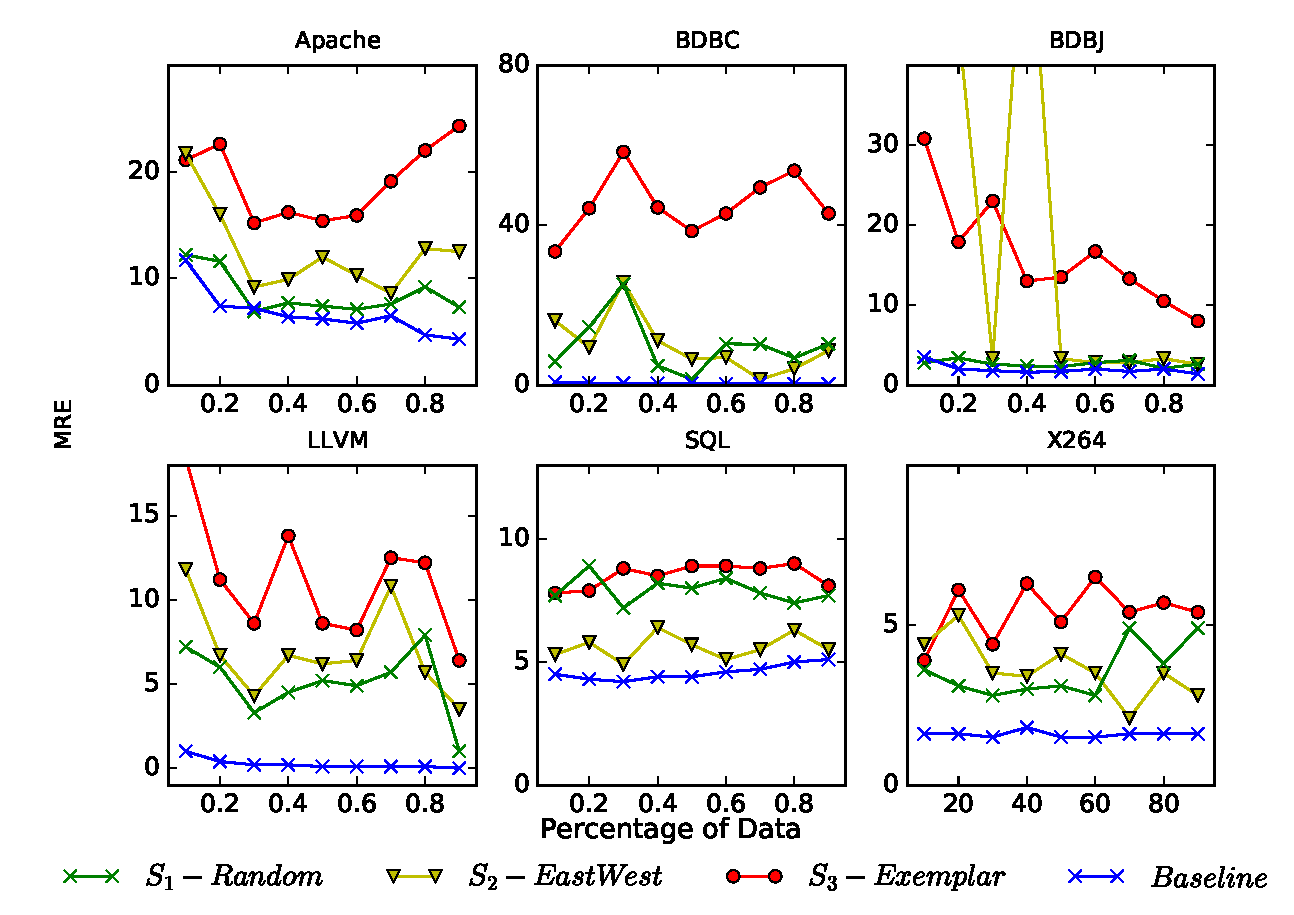
\includegraphics[width=\columnwidth]{Figures/SamplingAccuracy}
\caption{Errors of the predictions made by \what with four different
sampling policies. Note that, on the y-axis,  {\em lower} errors are {\em better}.
}
\label{fig:sampling_accuracy}
\end{figure}

\section{Results}
\subsection{RQ1}

\begin{center}
{\em Can  \what generate good predictions after
executing only a small number of configurations?}
\end{center}

\noindent Figure~\ref{sampling_accuracy} shows the mean errors of the predictors learned
after taking $X$\,\% of the configurations, then asking  \what and some sampling method ($S_1$, $S_2$, and $S_3$)
to (a)~find what configurations to measure; then (b)~asking CART to build a predictor
using these measurements. The horizontal axis of the plots shows what $X$\,\%
of the configurations are studied; the vertical axis shows the mean relative error (from \eq{err}).
In that figure:
\begin{itemize}
\item
The $\times$\hspace{-2pt}---\hspace{-2pt}$\times$ lines in Figure~\ref{sampling_accuracy} show a {\em baseline} result
where data from the performance scores of 100\,\% of  configurations were used by CART
to build a runtime predictor.
\item
The other lines show the results using the sampling methods defined in Section~\ref{sect:sample}.
Note that these sampling methods used  runtime data only from a
subset of 100\,\% of the performance scores seen in configurations
from 0 to X\,\%.
\end{itemize}

% \todo[inline]{PLEASE REMOVE - Actually, RQ1 does not say anything about varying the sampling policy; Furthermore, we have defined: \what =  WHERE $+$ $S_1$:Random $+$ CART, so \what plus S2... makes no sense. Vivek: I have changed the definition of WHAT to sampling policy because we are making a claim that any random point is better. Our recent studies have shown that using using outlier is not a good representative of a cluster}

In \fig{sampling_accuracy}, {\em lower} y-axis values  are {\em better} since this means lower
prediction errors. Overall, we find that:
\begin{itemize}

\item Some software systems exhibit large variances in their error rate, below $X=40$\,\% (e.g., BDBC and BDBJ).
\item Above $X=40$\,\%, there is little effect on the overall change of the sampling methods.
\item
Mostly, $S_3$ shows the highest overall error, 
so that it cannot be recommended.
\item Always, the   $\times$\hspace{-2pt}---\hspace{-2pt}$\times$ baseline shows the lowest errors, which is to be
expected since predictors built on the baseline have access to all data.
\item
We see a trend that the error of  $S_1$ and $S_2$ are within $5$\,\% of the {\em baseline} results.
Hence, we can recommend these two minimal sampling methods.
\end{itemize}

\begin{figure}[t]
\centering
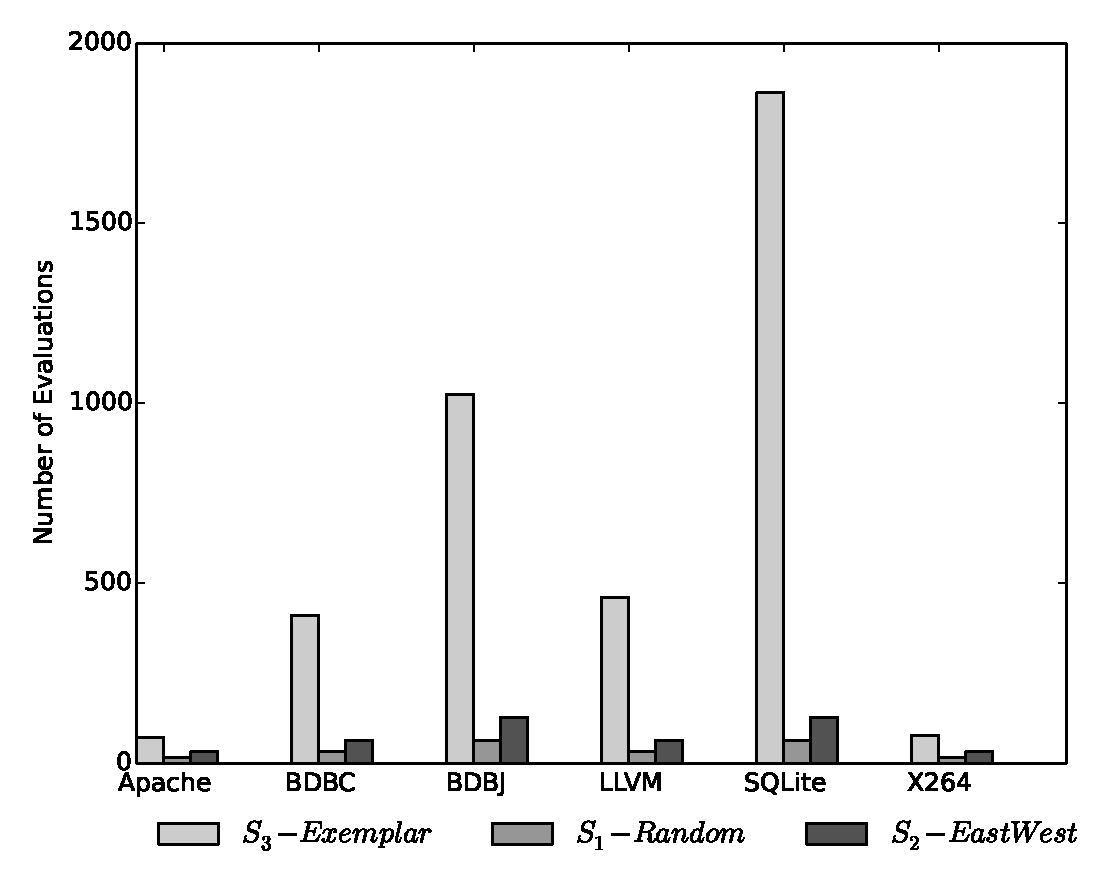
\includegraphics[width=0.75\columnwidth]{Figures/evaluation_graph}
\caption{Comparing evaluations of different sampling policies. We see that the number of configurations evaluated for $S_2$ is twice as high as $S_1$, as it selects 2 points from each cluster, where as  $S_1$ selects only 1 point. }\label{fig:Evaluations}
\end{figure}

\fig{Evaluations} provides information about which  of    $S_1$ or $S_2$ we should recommend.
This figure displays data taken from the $X=40$\,\% point of \fig{sampling_accuracy} and displays
how many performance scores of configurations are needed by our sub-sampling methods (while
reflecting on the configurations seen in the range $0\le X \le 40$). Note that:
\begin{itemize}
\item
$S_3$ needs up to thousands of performance-score points, 
so it cannot be recommended as minimal-sampling policy;
\item $S_2$ needs twice as much performance-score information as 
$S_1$ ($S_2$ uses {\em two} samples per leaf cluster  while
$S_1$ uses only {\em one}).
\item $S_1$ needs performance-score information on only a few dozen (or less) configurations to generate
the predictions with the lower errors seen in \fig{sampling_accuracy}.
\end{itemize}

Combining the results of \fig{sampling_accuracy} and \fig{Evaluations}, we conclude that:

\begin{myshadowbox}
$S_1$ is our preferred spectral sampling method. Furthermore,
the answer to {\bf RQ1} is ``yes'', because applying \what{}, we can (a)~generate runtime predictors
using just a few dozens of sample performance scores; 
and (b)~these predictions have error rates
within 5\,\% of the error rates seen if predictors are built from information about all performance scores.
\end{myshadowbox}




\subsection{RQ2}

\begin{center}
{\em
Do less data used in building models cause larger variances in the predicted values?}
\end{center}


Two competing effects can cause increased or decreased  variances in 
runtime predictions.
The   less we sample the configuration space,
the less we constrain model generation in that space. Hence, one effect that can be expected
is that models learned
from too few samples exhibit large variances. 
But,
a  compensating effect can be introduced by sampling from the spectral space
since that space contains fewer confusing or correlated variables than the raw configuration space.
\fig{Variance} reports which one of these two competing effects are dominant. 
\fig{sampling_accuracy} shows that after some initial fluctuations,
after seeing $X=40$\,\% of the configurations, the variances in prediction errors reduces to nearly zero.


\begin{figure}[tbh]
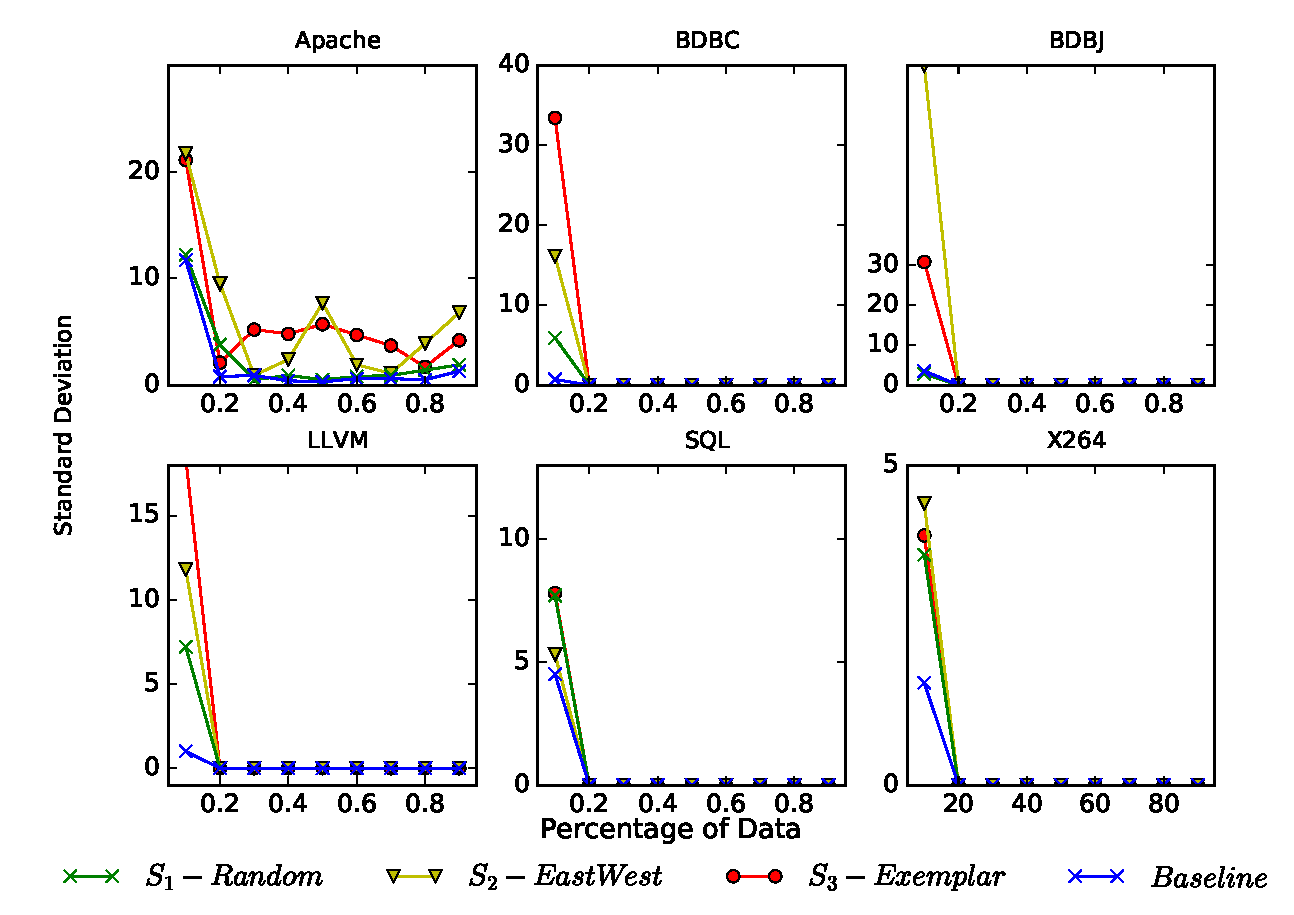
\includegraphics[width=\columnwidth]{Figures/Variance}
\centering
\caption{Standard deviations seen at various points of  \fig{sampling_accuracy}.}\label{fig:Variance}
\end{figure}

\begin{myshadowbox}
Hence, we answer {\bf RQ2} with ``no'': Selecting a small number of samples does not necessarily increase variance (at least to say, not in this domain).
\end{myshadowbox}


\subsection{RQ3}

\begin{center}
{\em
Can ``good'' surrogate models (to be used in optimizers)
be built from minimal samples?}
\end{center}

The results of answering {\bf RQ1} and {\bf RQ2} suggest to use \what (with $S_1$) to build runtime predictors from a small sample of  data. {\bf RQ3}
asks if that predictor can be used by an optimizer to infer what {\em other} configurations correspond to system configurations with fast performance scores.
To answer this question,  we ran  a random set of 100 
configurations, 20 times, and related that baseline to three optimizers (GALE~\cite{krall2014gale}, DE~\cite{storn1997differential} and  NSGA-II~\cite{deb00afast}) using their
default parameters.
 
When these three optimizers mutated existing configurations to suggest new ones,
these mutations were checked for validity. Any mutants that violated the system's constraints (e.g., a feature excluding another feature) were rejected
and the survivors were ``evaluated'' by asking the CART surrogate model.
%(the  CART regression-tree learned from \what+$S_1$:Random, built using the methods of {\bf RQ1}).
These evaluations either rejected the mutant or used it in generation $i+1$, as the basis for a search for more, possibly
better  mutants.




\fig{performance_graph} shows the configurations found by three optimizers projected onto the ground truth of the performance scores of nearly
all configurations (see Section~\ref{sec:subject_systems}). Again note that, while we use that ground truth for the validation of these results, our optimizers 
used only a small part of that ground-truth data in their search for the fastest configurations (see the \what + $S_1$
results of \fig{Evaluations}).


\begin{figure}[tb]
\centering
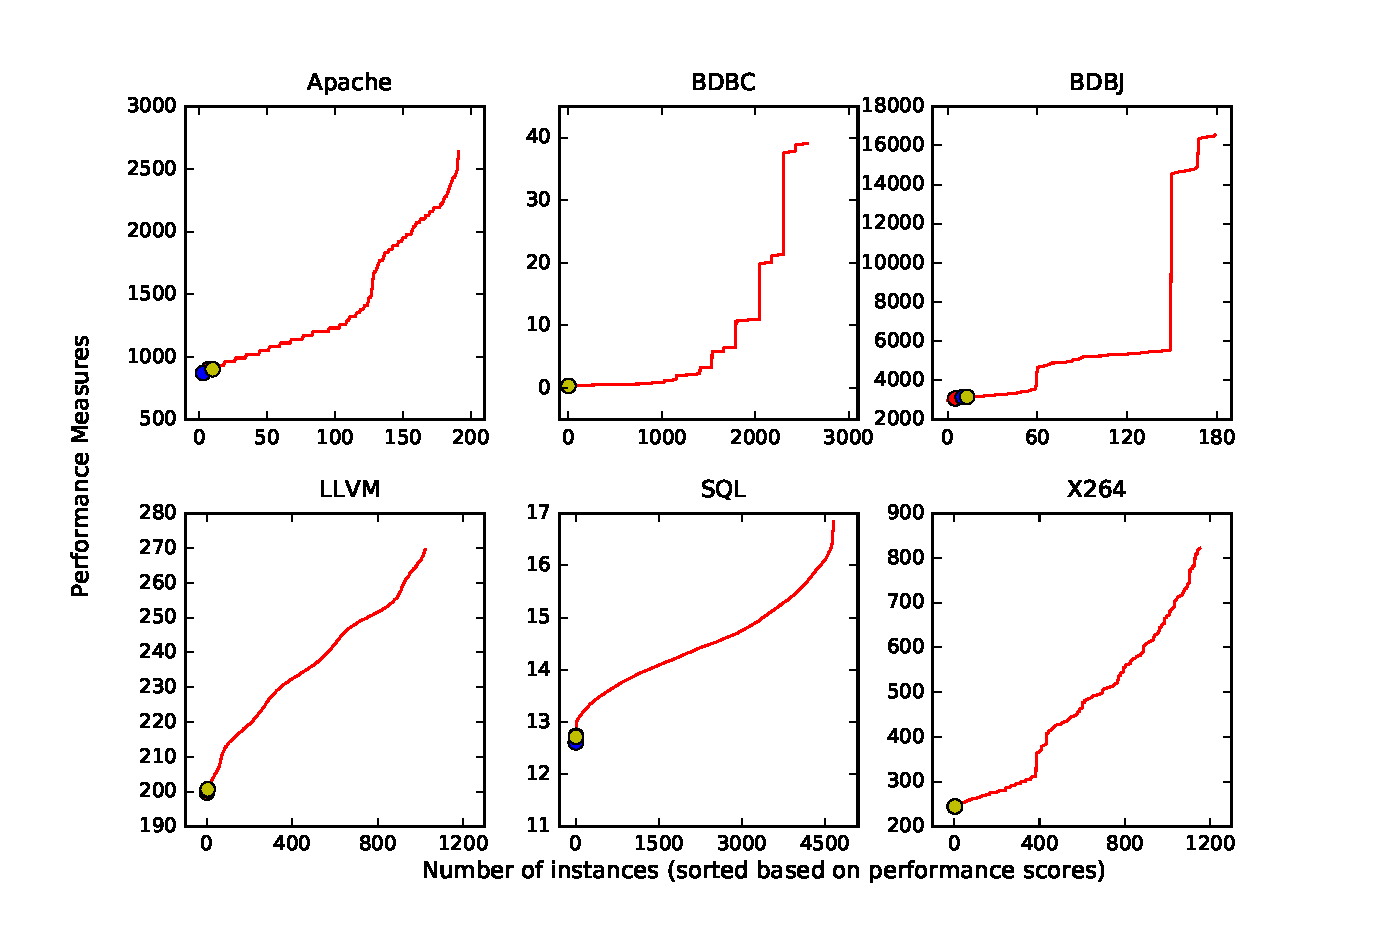
\includegraphics[width=\columnwidth]{Figures/optimizer_result}
\caption{Solutions found by GALE, NSGA-II and DE (shown as points) laid against the ground truth (all known configuration performance scores). 
% In case of Apache and BDBJ, we can see that the different optimizers find different solutions but in the remaining plots, the results are the same. 
It can be observed that all the optimizers can find the configuration with  lower performance scores.}\label{fig:performance_graph}
\end{figure}


The important feature of \fig{performance_graph} is that all the optimized configurations fall within 1\,\% of the fastest
configuration according to the ground truth (see all the left-hand-side dots on each plot). Table~\ref{fig:external_validity} compares the performance of the optimizers
used in this study. Note that the performances are nearly identical, which leads to the following conclusions:

\begin{myshadowbox}
The answer to {\bf RQ3} is ``yes'': For optimizing performance scores, we can use surrogates built from few runtime samples. The choice of the optimizer does not critically effect this conclusion.
\end{myshadowbox}


\begin{table}[tbh]
\centering
\caption{The table shows how the minimum performance scores as found by the learners GALE, NSGA-II, and DE, vary over 20 repeated
runs. Mean values are denoted $\mu$ and IQR denotes the 25th--75th percentile. A low IQR suggests that the surrogate model build by \what is stable and can be utilized by off the shelf optimizers to find performance-optimal configurations.
% \todo[inline]{$\mu$ is reserved for the mean of the entire population, not for the mean of the part of the data we look at.}
}
\label{fig:external_validity}
\vspace{2ex}
\begin{tabular}{lrrrrrr}
\toprule
\multirow{3}{*}{\textbf{Dataset}} & \multicolumn{6}{c}{\textbf{Searcher}}                                                                       \\ \cmidrule{2-7} 
                                  & \multicolumn{2}{c}{\textbf{GALE}} & \multicolumn{2}{c}{\textbf{DE}} & \multicolumn{2}{c}{\textbf{NSGAII}} \\ \cmidrule{2-7} 
                                  & \textbf{Mean}    & \textbf{IQR}    & \textbf{Mean}   & \textbf{IQR}   & \textbf{Mean}     & \textbf{IQR}     \\ \midrule
\textbf{Apache}                   & 870              & 0               & 840             & 0              & 840               & 0                \\ 
\textbf{BDBC}                     & 0.363            & 0.004           & 0.359           & 0.002          & 0.354             & 0.005            \\ 
\textbf{BDBJ}                     & 3139             & 70              & 3139            & 70             & 3139              & 70               \\ 
\textbf{LLVM}                     & 202              & 3.98            & 200             & 0              & 200               & 0                \\ 
\textbf{SQLite}                   & 13.1             & 0.241           & 13.1            & 0              & 13.1              & 0.406            \\ 
\textbf{X264}                     & 248              & 3.3             & 244             & 0.003          & 244               & 0.05             \\ \bottomrule
\end{tabular}
\end{table}

% \begin{figure*}[tbh]
% 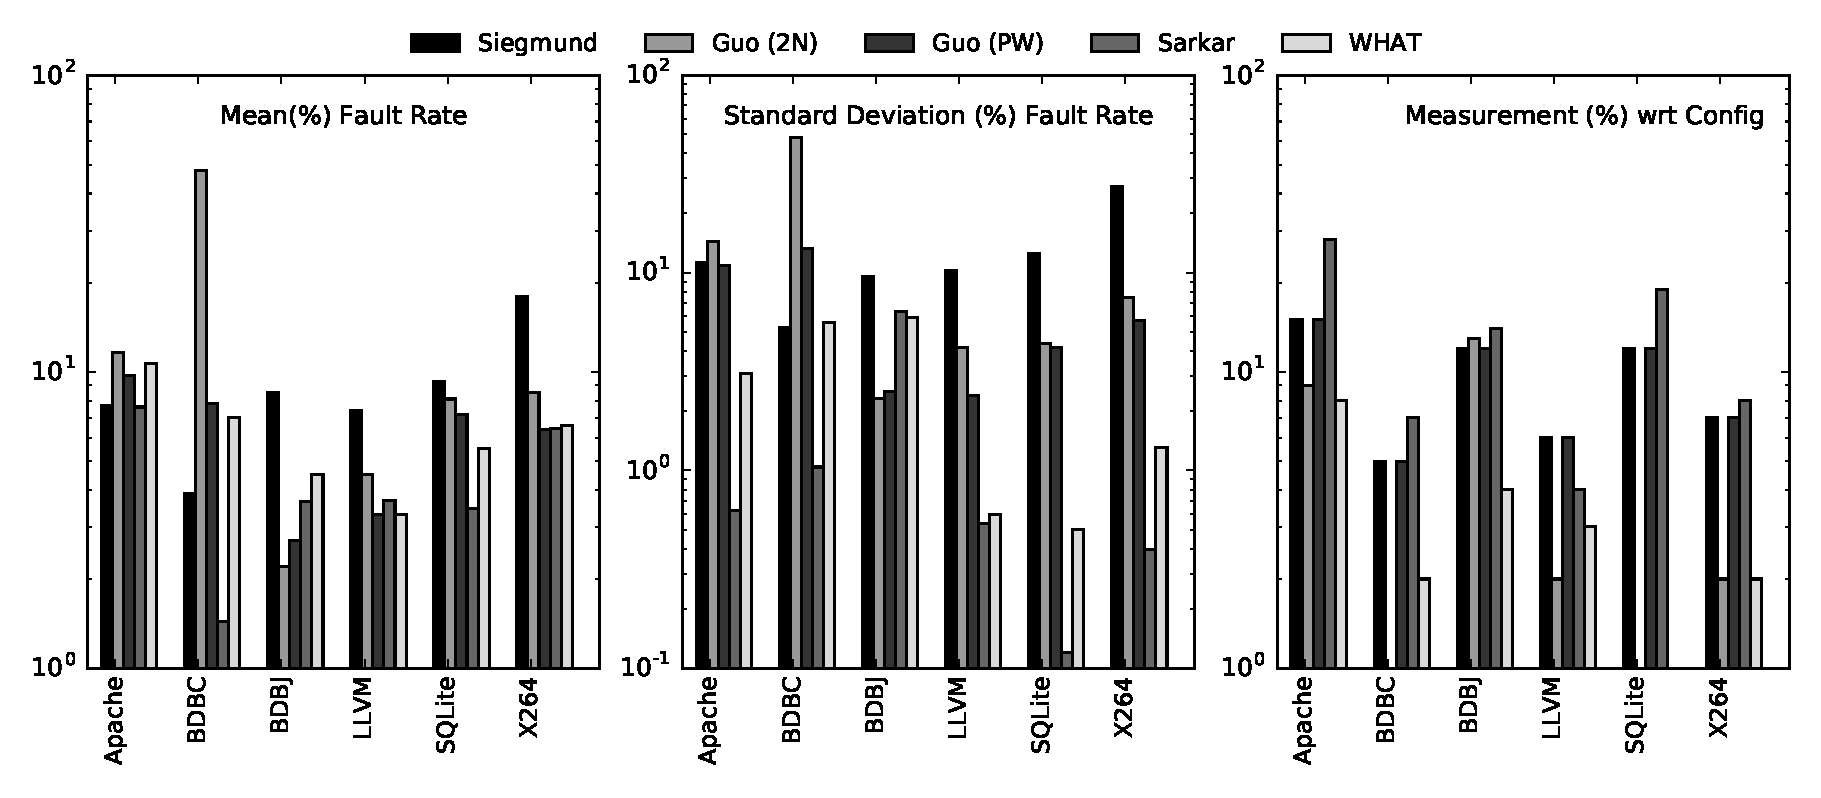
\includegraphics[width=\linewidth]{Figures/compare_graph_h}
% \caption{Comparison between \what and the state-of-the-art approaches regarding mean error, standard deviation, and the percentage of configurations used for training the model.} \label{fig:Comparison}
% % \todo[inline]{Please use different brightness/alpha values or patterns to be able to distinguish the bar on a print out.}
% \end{figure*}
 
 
\begin{figure*}[h]
 \begin{minipage}{4in}

        {\small
          \begin{tabular}{l@{~~~~}l@{~~~~}r@{~~~~}r@{~~}c@{}r}
    
    
  \multicolumn{1}{l}{\textbf{Rank}}& \textbf{using} & \textbf{Mean MRE}& \textbf{STDev} & \textbf{} & \textbf{Evaluations} \\ 
 \rowcolor{lightgray}\arrayrulecolor{lightgray}
\textbf{Apache}  & \textbf{} & \textbf{} & \textbf{}&\textbf{}&  \\\hline
  1 &       Sarkar &    7.49  &  0.82 & \quart{6}{3}{7} & 55 \\
  1 &      Guo(PW) &    10.51  &  6.85 & \quart{3}{33}{22} & 29 \\
  1 &     Siegmund &    10.34  &  11.68 & \quart{0}{55}{21} &  29\\
  1 &         	\textbf{WHAT} &    10.95  &  2.74 & \quart{16}{13}{24} & 16 \\
  1 &      Guo(2N) &    13.03  &  15.28 & \quart{7}{72}{34} &  18\\
\hline  
\rowcolor{lightgray}\arrayrulecolor{lightgray}
\textbf{BDBC}  & \textbf{} & \textbf{} & \textbf{}& \textbf{}&\\\hline
  1 &       Sarkar &    1.24  &  1.46 & \quart{0}{1}{0} &  191\\
\hline  2 &     Siegmund &    6.14  &  4.41 & \quart{4}{5}{6} &  139\\
  2 &         	\textbf{WHAT} &    6.57  &  7.4 & \quart{4}{9}{7} &  64\\
  2 &      Guo(PW) &    10.16  &  10.6 & \quart{2}{13}{11} &  139\\
\hline  3 &      Guo(2N) &    49.9  &  52.25 & \quart{16}{63}{59} &  36\\
\hline  
\rowcolor{lightgray}\arrayrulecolor{lightgray}
\textbf{BDBJ}  & \textbf{} & \textbf{} & \textbf{}& \textbf{}&\\\hline
  1 &      Guo(2N) &    2.29  &  3.26 & \quart{0}{29}{9} &  52\\
  1 &      Guo(PW) &    2.86  &  2.72 & \quart{2}{25}{14} &  48\\
  1 &         	\textbf{WHAT} &    4.75  &  4.46 & \quart{12}{40}{31} &  16\\
\hline  2 &       Sarkar &    5.67  &  6.97 & \quart{6}{62}{39} &  48\\
  2 &     Siegmund &    6.98  &  7.13 & \quart{16}{63}{51} &  57\\
\hline  
\rowcolor{lightgray}\arrayrulecolor{lightgray}
\textbf{LLVM}  & \textbf{} & \textbf{} & \textbf{}&\textbf{}& \\\hline
  1 &      Guo(PW) &    3.09  &  2.98 & \quart{0}{21}{10} &  64\\
  1 &         	\textbf{WHAT} &    3.32  &  1.05 & \quart{9}{7}{12} &  32\\
  1 &       Sarkar &    3.72  &  0.45 & \quart{13}{3}{15} &  62\\
  1 &      Guo(2N) &    4.99  &  5.05 & \quart{11}{36}{24} &  22\\
\hline  2 &     Siegmund &    8.5  &  8.28 & \quart{21}{58}{49} &  43\\
\hline
 
 
\rowcolor{lightgray}\arrayrulecolor{lightgray}
\textbf{SQLite} & \textbf{} & \textbf{} & \textbf{} & \textbf{}&\\\hline
  1 &       Sarkar &    3.44  &  0.1 & \quart{0}{0}{0} &  925\\
\hline  2 &         	\textbf{WHAT} &    5.6  &  0.57 & \quart{7}{2}{8} &  64\\
\hline  3 &      Guo(2N) &    8.57  &  7.3 & \quart{2}{28}{19} &  78\\
  3 &      Guo(PW) &    8.94  &  6.24 & \quart{6}{24}{20} &  566\\
\hline  4 &     Siegmund &    12.83  &  17.0 & \quart{16}{63}{35} &  566\\
\hline  
\rowcolor{lightgray}\arrayrulecolor{lightgray}
\textbf{x264} & \textbf{} & \textbf{} & \textbf{}& \textbf{}&\\\hline
  1 &       Sarkar &    6.64  &  1.04 & \quart{4}{2}{5} &  93\\
  1 &         	\textbf{WHAT} &    6.93  &  1.67 & \quart{4}{4}{6} &  32\\
  1 &      Guo(2N) &    7.18  &  7.07 & \quart{0}{15}{6} &  32\\
  1 &      Guo(PW) &    7.72  &  2.33 & \quart{4}{5}{8} &  81\\
\hline  2 &     Siegmund &    31.87  &  21.24 & \quart{32}{47}{61} &  81\\
\hline 

  \end{tabular}} 
\end{minipage}
\caption{Mean MRE seen in 20 repeats. Mean MRE is the prediction error as described in Equation~\ref{eq:err} and STDev is the standard deviation of the MREs found during multiple repeats. 
Lines with a a dot in the middle 
(e.g. \protect \quartex{3}{13}{13}) 
show the mean as a round dot withing the IQR (and if the IQR is very small, only a  round dot will be visible). 
All the results are sorted by the mean values: lower mean value of MRE is better than large mean value. 
The left-hand side columns \textbf{Rank} the various techniques, smaller the value of \textbf{Rank} better the technique e.g. in Apache, all the techniques have the same rank since their mean values are not statistically different. \textbf{Rank} is computer using Scott-Knott, bootstrap 95\% confidence, and the A12 test.
}
\label{fig:stats}
\end{figure*} 
 
 
\subsection{RQ4}


% \todo[inline]{change fault rate to error rate. note the sampling heuristic used for siegmund (I guess FW?!)}

 \begin{center}
{\em How good is \what compared to the state of the art of learning performance predictors from configurable software systems?}
\end{center}

We compare \what with the three state-of-the-art predictors proposed in the literature~\cite{siegmund2012predicting}, \cite{guo2013variability}, \cite{sarkar2015cost}, as discussed in Section~\ref{sect:addit}. Note that all approaches use regression-trees as predictors, except Siegmund's approach, which uses a regression function derived using linear programming.
The results were studied using non-parametric tests, which was also used by Arcuri and Briand at ICSE
'11~\cite{mittas13}). For testing statistical significance,
we used non-parametric bootstrap test 95\% confidence~\cite{efron93} followed by
an A12 test to check that any observed differences were not trivially small effects;
i.e. given two lists $X$ and $Y$, count how often there are larger
numbers in the former list (and there there are ties, add a half mark):
$a=\forall x\in X, y\in Y\frac{\#(x>y) + 0.5*\#(x=y)}{|X|*|Y|}$
(as per Vargha~\cite{Vargha00}, we say that a ``small'' effect has $a <0.6$). 
Lastly, to generate succinct reports, we use the Scott-Knott test to recursively
divide our optimizers. This recursion used A12 and bootstrapping  
to group together subsets that are (a)~not significantly different and are (b)~not
just a small effect different to each other. This use of Scott-Knott is endorsed
by Mittas and Angelis~\cite{mittas13}
and by Hassan et al.~\cite{7194626}.

As seen in the Figure~\ref{fig:stats}, the FW approach of Siegmund et al. (i.e., the sampling approach using the fewest number of configurations) $(4/6)$ times has the higher errors rate and the highest standard deviation on that error rate. Hence, we cannot recommend this method or, if one wishes to use this method, we recommend using the other sampling heuristics (e.g., HO, HS) to make more accurate predictions (but at the cost of much more measurements). Moreover, the size of the standard deviation of this method causes further difficulties in estimating which configurations are those exhibiting a large prediction error. 

THere are two cases in Figure~\ref{fig:stats} where \what performs worse than at least one
other methods:
\begin{itemize}
\item 
SQLite: here, the Sukar methods does better that \what (3.44 vs 5.6)
but, as shown in the final column of Figure~\ref{fig:stats},
does so at the cost of $\frac{925}{64} \approx 15$ times more evaluations that \what.
In this case, a pragmatic engineering could well prefer our solution the that of Sukar (since
Sukar uses  more than an order of magnitude slowdown).
\item BDBC: Here again, \what is not doing the best but, compared to the space of
all other solutions, it  is not doing particular bad.
\end{itemize}


As to the approach of Guo et al (with PW), this does not standout on any of our measurements. Its error results are within 1\% of \what; its standard deviation are usually larger and it requires much more data than \what (Evaluations column of the figure). 

In terms of the number of measure samples required to build a model, the right-hand most column of Figure~\ref{fig:stats} shows that \what requires the fewest samples except for two cases: the approach of Guo et al. (with 2N) working on BDBC and LLVM. In both these cases, the mean error and standard deviation on the error estimate is larger than \what. Furthermore, in the case of BDBC, the error values
 are $\mu=14\,\%$, $\sigma=13\,\%$, which are much larger
than \what{}'s error scores of $\mu=6\,\%$, $\sigma=5\,\%$.

Although the approach of Sarkar et al. produces an error rate that is sometimes less than the one of \what, it requires the most number of measurements. Moreover, \what\'s  accuracy is close to Sarkar\'s approach (1\% to 2\%) difference). Hence, we cannot recommend this approach, too.

Table~\ref{tab:measurements} shows the number of evaluations used by each approaches. We see that most state-of-the-art approaches often require many more samples than
\what{}.  Using those fewest numbers of samples, \what has
within 1 to 2\,\% of the lowest standard deviation rates 
and within 1 to 2\,\% of lowest error rates.
The exception is Sarkar's approach, which has 5\,\% lower mean error
rates (in BDBC, see the left-hand-side plot of Figure~\ref{fig:Comparison}).  However, 
as shown in right-hand-side of Table~\ref{tab:measurements}, Sarkar's approach needs nearly three times
more measurements than \what (191 vs 64 samples). Given
the overall reduction of the error is   small (5\,\% difference
between Sarkar and \what in mean error), the overall
cost of tripling the data-collection cost is
often not feasible in a practical context and might not justify the small additional benefit in accuracy. 

%  The \framebox{\colorbox{whatcolor}{\textcolor{whatcolor}{\bf blue}}} bars of Figure \ref{fig:Comparison} show the
%  mean error rate, the standard deviation of the error rate, and the mean percentage
%  of total configurations used in 30 repeats of the different approaches.
%  Note that the y-axis of that figure is a logarithmic scale so, within each plot:
%  \begin{itemize}
%  \item Differences near the bottom  are very small differences;
%  \item Differences near the top   are very large differences;
%  \end{itemize}
 
% As seen in the left and middle plots of
% Figure~\ref{fig:Comparison}, 
% the {\em FW} approach of Siegmund et al.\ (i.e., the sampling approach using the fewest number of configurations) often has the highest
% error rate and the highest
% standard deviation on that error rate. Hence,
% we cannot recommend this method or,  if one wishes to use this method, we recommend using the other sampling heuristics (e.g., HO, HS) to make more accurate predictions (but at the cost of much more measurements). Moreover, the size of the standard deviation of this method causes further difficulties in estimating which configurations are those exhibiting a large prediction error. 

% As to the approach of Guo et al.\ (with PW), this   does not standout on any of
% our measurements. Its error results are within 1\,\% of \what;
%  its standard deviation are usually larger; and it requires
%  much more data than \what.
 
%  In terms of the number of measured samples required to build a model, 
%  the right-hand-side plot of  Figure~\ref{fig:Comparison}  shows that
%  \what requires the fewest samples except for two cases:
%  the approach of Guo et al. (with 2N) working on BDBC and LLVM.  In both these cases, the mean error and standard deviation on the error
%  estimate is   larger than \what  (see the \framebox{\colorbox{guocolor}{\textcolor{guocolor}{\bf red}}} bars in the left and middle plots   of Figure~\ref{fig:Comparison}). Furthermore, in the case of BDBC, the error values
%  are $\mu=14\,\%$, $\sigma=13\,\%$, which are much larger
% than \what{}'s error scores of $\mu=6\,\%$, $\sigma=5\,\%$. 


% Although the approach of Sarkar et al.\ produces an error rate that is sometimes less than the one of \what (see the left-hand-side of
% Figure~\ref{fig:Comparison}), it requires the most number of measurements. Moreover, \what's accuracy is close to Sarkar's approach (1\,\%
% to 2\,\% difference). Hence, we cannot recommend this approach, too.

% %Nor can we recommend the approach of Sarkar et al.\ since,
% %as shown on the right-hand-side of Figure~\ref{fig:Comparison}, 
% %this approach requires the most data.
% %While it is true that its error rate 
% %is sometimes less than the one of \what (see the left-hand-side of
% %Figure~\ref{fig:Comparison}), that difference is often small (1\,\%
% %to 2\,\%). 

% %The exception here is BDBC, where Sarker's approach has the lowest
% %error of any approach. This exception is discussed further in the
% %next paragraph.
 

% The right-hand-side of Figure~\ref{fig:Comparison}   shows
% the {\em percent} of required measurements. Table~\ref{tab:measurements} shows the same
% expressed as absolute values. We see that most state-of-the-art approaches often require many more samples than
% \what{}.  Using those fewest numbers of samples, \what has
% within 1 to 2\,\% of the lowest standard deviation rates 
% and within 1 to 2\,\% of lowest error rates.
% The exception is Sarkar's approach, which has 5\,\% lower mean error
% rates (in BDBC, see the left-hand-side plot of Figure~\ref{fig:Comparison}).  However, 
% as shown in right-hand-side of Table~\ref{tab:measurements}, Sarkar's approach needs nearly three times
% more measurements than \what (191 vs 64 samples). Given
% the overall reduction of the error is   small (5\,\% difference
% between Sarkar and \what in mean error), the overall
% cost of tripling the data-collection cost is
% often not feasible in a practical context and might not justify the small additional benefit in accuracy. 


 %Note that:
%  \bi
%     \item
    
%  \ei




\begin{table}[t]
\caption{Comparison of the number of the samples
required with the state of the art. The grey colored cells indicate the approach which has the lowest number of samples.  We notice that WHAT and Guo (2N) uses less data compared to other approaches. The high fault rate  of Guo (2N) accompanied with high variability in the predictions makes WHAT our preferred method.}\label{tab:measurements}
\vspace{2ex}
\centering
\small
\begin{tabular}{lrrrrr}
\toprule
                                   & \multicolumn{5}{c}{\textbf{Samples}}                                                                         \\ \cmidrule{2-6} 
\multirow{-2}{*}{\textbf{Dataset}} & \textbf{Siegmund} & \textbf{Guo (2N)}          & \textbf{Guo (PW)} & \textbf{Sarkar} & \textbf{\what}                \\ \midrule
\textbf{Apache}                    & 29                & 181                        & 29                & 55              & \cellcolor[HTML]{C0C0C0}16 \\ 
\textbf{BDBC}                      & 139               & \cellcolor[HTML]{C0C0C0}36 & 139               & 191             & 64                         \\ 
\textbf{BDBJ}                      & 48                & 52                         & 48                & 57              & \cellcolor[HTML]{C0C0C0}16 \\ 
\textbf{LLVM}                      & 62                & \cellcolor[HTML]{C0C0C0}22 & 64                & 43              & 32                         \\ 
\textbf{SQLite}                    & 566               & 78                         & 566               & 925             & \cellcolor[HTML]{C0C0C0}64 \\ 
\textbf{X264}                      & 81                & \cellcolor[HTML]{C0C0C0}32 & 81                & 93              & \cellcolor[HTML]{C0C0C0}32 \\ \bottomrule
\end{tabular}
\end{table}

% % Please add the following required packages to your document preamble:
% \usepackage{multirow}
% \usepackage[table,xcdraw]{xcolor}
% If you use beamer only pass "xcolor=table" option, i.e. \documentclass[xcolor=table]{beamer}
\begin{figure*}[!t]
\centering
\begin{tabular}{|l|l|l|l|l|l|l|l|}
\hline
                                   & \multicolumn{2}{c|}{}                                             &                                            & \multicolumn{2}{l|}{\thead{FaultRate(Them) \\ Siegmund et al.}}               & \multicolumn{2}{l|}{\thead{FaultRate(US) \\ This paper}}   \\ \cline{5-8} 
\multirow{-2}{*}{\thead{Dataset}} & \multicolumn{2}{c|}{\multirow{-2}{*}{\thead{Measurement(Them) \\ Siegmund et al. \\}}} & \multirow{-2}{*}{\thead{Measurement(Us) \\ This paper \\}} & \thead{Mean}                & \thead{Std}                 & \thead{Mean}         & \thead{Std}          \\ \hline
                                   & FW                              & 15                              &                                            & \cellcolor[HTML]{C0C0C0}44.1 & \cellcolor[HTML]{C0C0C0}42.3 &                       &                       \\ \cline{2-3} \cline{5-6}
                                   & PW                              & \cellcolor[HTML]{FD6864}139                             &                                            & 3.9                          & 5.3                          &                       &                       \\ \cline{2-3} \cline{5-6}
                                   & HO                              & \cellcolor[HTML]{FD6864}160                             &                                            & 2.8                          & 3.7                          &                       &                       \\ \cline{2-3} \cline{5-6}
\multirow{-4}{*}{BDBC}             & HS                              & \cellcolor[HTML]{FD6864}164                             & \multirow{-4}{*}{64}                       & 2.8                          & 3.7                          & \multirow{-4}{*}{9.3} & \multirow{-4}{*}{6.8} \\ \hline
                                   & FW                              & 10                              &                                            & \cellcolor[HTML]{C0C0C0}17.7 & \cellcolor[HTML]{C0C0C0}19.6 &                       &                       \\ \cline{2-3} \cline{5-6}
                                   & PW                              & 48                              &                                            & \cellcolor[HTML]{C0C0C0}8.5  & \cellcolor[HTML]{C0C0C0}9.6  &                       &                       \\ \cline{2-3} \cline{5-6}
                                   & HO                              & \cellcolor[HTML]{FD6864}116                             &                                            & \cellcolor[HTML]{C0C0C0}3.8  & \cellcolor[HTML]{C0C0C0}5.7  &                       &                       \\ \cline{2-3} \cline{5-6}
\multirow{-4}{*}{BDBJ}             & HS                              & \cellcolor[HTML]{FD6864}162                             & \multirow{-4}{*}{64}                       & 1.7                          & 3.5                          & \multirow{-4}{*}{2.7} & \multirow{-4}{*}{0.7} \\ \hline
                                   & FW                              & 9                               &                                            & \cellcolor[HTML]{C0C0C0}14.9 & \cellcolor[HTML]{C0C0C0}24.8 &                       &                       \\ \cline{2-3} \cline{5-6}
                                   & PW                              & \cellcolor[HTML]{FD6864}29                              &                                            & \cellcolor[HTML]{C0C0C0}7.7  & \cellcolor[HTML]{C0C0C0}11.2 &                       &                       \\ \cline{2-3} \cline{5-6}
                                   & HO                              & \cellcolor[HTML]{FD6864}80                              &                                            & \cellcolor[HTML]{C0C0C0}11.6 & \cellcolor[HTML]{C0C0C0}22.7 &                       &                       \\ \cline{2-3} \cline{5-6}
\multirow{-4}{*}{Apache}           & HS                              & \cellcolor[HTML]{FD6864}143                             & \multirow{-4}{*}{16}                       & 5.3                          & 10.8                         & \multirow{-4}{*}{9.9} & \multirow{-4}{*}{2.4} \\ \hline
                                   & FW                              & 26                              &                                            & \cellcolor[HTML]{C0C0C0}7.8  & \cellcolor[HTML]{C0C0C0}9.2  &                       &                       \\ \cline{2-3} \cline{5-6}
                                   & PW                              & \cellcolor[HTML]{FD6864}566                             &                                            & \cellcolor[HTML]{C0C0C0}9.3  & \cellcolor[HTML]{C0C0C0}12.5 &                       &                       \\ \cline{2-3} \cline{5-6}
                                   & HO                              & \cellcolor[HTML]{FD6864}566                             &                                            & \cellcolor[HTML]{C0C0C0}7.1  & \cellcolor[HTML]{C0C0C0}9.1  &                       &                       \\ \cline{2-3} \cline{5-6}
\multirow{-4}{*}{SQL}              & HS                              & \cellcolor[HTML]{FD6864}569                             & \multirow{-4}{*}{64}                       & \cellcolor[HTML]{C0C0C0}7    & \cellcolor[HTML]{C0C0C0}9    & \multirow{-4}{*}{5.6} & \multirow{-4}{*}{0.2} \\ \hline
                                   & FW                              & 11                              &                                            & \cellcolor[HTML]{C0C0C0}7.8  & \cellcolor[HTML]{C0C0C0}9    &                       &                       \\ \cline{2-3} \cline{5-6}
                                   & PW                              & \cellcolor[HTML]{FD6864}62                              &                                            & \cellcolor[HTML]{C0C0C0}7.4  & \cellcolor[HTML]{C0C0C0}10.2 &                       &                       \\ \cline{2-3} \cline{5-6}
                                   & HO                              & \cellcolor[HTML]{FD6864}62                              &                                            & \cellcolor[HTML]{C0C0C0}7.4  & \cellcolor[HTML]{C0C0C0}10.2 &                       &                       \\ \cline{2-3} \cline{5-6}
\multirow{-4}{*}{LLVM}             & HS                              & \cellcolor[HTML]{FD6864}88                              & \multirow{-4}{*}{32}                       & \cellcolor[HTML]{C0C0C0}5.7  & \cellcolor[HTML]{C0C0C0}7    & \multirow{-4}{*}{3.3} & \multirow{-4}{*}{0.3} \\ \hline
                                   & FW                              & 12                              &                                            & \cellcolor[HTML]{C0C0C0}29.8 & \cellcolor[HTML]{C0C0C0}22   &                       &                       \\ \cline{2-3} \cline{5-6}
                                   & PW                              & \cellcolor[HTML]{FD6864}81                              &                                            & \cellcolor[HTML]{C0C0C0}17.9 & \cellcolor[HTML]{C0C0C0}27.2 &                       &                       \\ \cline{2-3} \cline{5-6}
                                   & HO                              & \cellcolor[HTML]{FD6864}89                              &                                            & 5.1                          & 15.1                         &                       &                       \\ \cline{2-3} \cline{5-6}
\multirow{-4}{*}{x264}             & HS                              & \cellcolor[HTML]{FD6864}89                              & \multirow{-4}{*}{32}                       & 5.1                          & 15.1                         & \multirow{-4}{*}{6.6} & \multirow{-4}{*}{0.5} \\ \hline
\end{tabular}
\caption{Comparison of
Seigmund et.al \cite{siegmund2012predicting} with WHAT+$S_1$:Random 
(shown in right-hand columns). Gray   denote cases where prior work has larger median error. Red test denotes all cases where prior work used large samples. Note that in all cases where prior work achieved lower mean error rate, they required more samples for ex. in Apache HS 143 samples to 16 samples with our method.
}\label{fig:vs2012}
\end{figure*}

% % Please add the following required packages to your document preamble:
% \usepackage[table,xcdraw]{xcolor}
% If you use beamer only pass "xcolor=table" option, i.e. \documentclass[xcolor=table]{beamer}
\begin{figure*}[!t]
\centering
\begin{tabular}{|l|l|l|l|l|l|l|}
\hline
\thead{Dataset} & \thead{Mean Fault \\ Rate(Guo)} & \thead{Standard \\ Deviation(Guo)}   & \thead{Measurement \\ (Guo)} & \thead{Mean Fault \\ Rate(Us)} & \thead{Standard \\ Deviation(Us)} & \thead{Measurement \\ (Us)} \\ \hline
\textbf{Apache}  & \cellcolor[HTML]{C0C0C0}11.6  & \cellcolor[HTML]{C0C0C0}14.4  & \cellcolor[HTML]{C0C0C0}18 & 9.9                          & 2.4                         & 16                         \\ \hline
\textbf{LLVM}    & \cellcolor[HTML]{C0C0C0}4.5   & \cellcolor[HTML]{C0C0C0}4.2   & 22                         & 3.3                          & 0.3                         & 32                         \\ \hline
\textbf{X264}    & \cellcolor[HTML]{C0C0C0}8.5   & \cellcolor[HTML]{C0C0C0}7.5   & \cellcolor[HTML]{C0C0C0}32 & 6.6                          & 0.5                         & 32                         \\ \hline
\textbf{BDBC}    & \cellcolor[HTML]{C0C0C0}98.3  & \cellcolor[HTML]{C0C0C0}243.1 & 36                         & 9.3                          & 6.8                         & 64                         \\ \hline
\textbf{BDBJ}    & 2.2                           & \cellcolor[HTML]{C0C0C0}2.3   & 52                         & 2.7                          & 0.7                         & 64                         \\ \hline
\textbf{SQLite}  & \cellcolor[HTML]{C0C0C0}8.1   & \cellcolor[HTML]{C0C0C0}4.4   & \cellcolor[HTML]{C0C0C0}78 & 5.6                          & 0.2                         & 64                         \\ \hline
\end{tabular}
\caption{Comparison of
Guo et.al \cite{guo2013variability}, which uses $2*N$ number of configurations with WHAT + $S_1$ 
(shown in right-hand columns). Here N refers to the number of features of the software system (please refer to \cite{guo2013variability} for more details).  Gray denotes the cases where our method results in lower median fault rate and is more stable i.e. lower standard deviation. We see that our method does better in 3 out of 6 datasets. }\label{fig:guo_2n}
\end{figure*}

% % Please add the following required packages to your document preamble:
% \usepackage[table,xcdraw]{xcolor}
% If you use beamer only pass "xcolor=table" option, i.e. \documentclass[xcolor=table]{beamer}
\begin{figure*}[!t]
\centering
\begin{tabular}{|l|l|l|l|l|l|l|}
\hline
\thead{Dataset} & \thead{Mean Fault \\ Rate(Guo)} & \thead{Standard \\ Deviation(Guo)}   & \thead{Measurement \\ (Guo)} & \thead{Mean Fault \\ Rate(Us)} & \thead{Standard \\ Deviation(Us)} & \thead{Measurement \\ (Us)} \\ \hline
\textbf{Apache}  & 9.7                           & \cellcolor[HTML]{C0C0C0}10.8 & \cellcolor[HTML]{C0C0C0}29  & 9.9                          & 2.4                         & 16                         \\ \hline
\textbf{LLVM}    & 3.3                           & \cellcolor[HTML]{C0C0C0}2.4  & \cellcolor[HTML]{C0C0C0}64  & 3.3                          & 0.3                         & 32                         \\ \hline
\textbf{X264}    & 6.4                           & \cellcolor[HTML]{C0C0C0}5.7  & \cellcolor[HTML]{C0C0C0}81  & 6.6                          & 0.5                         & 32                         \\ \hline
\textbf{BDBC}    & 7.8                           & \cellcolor[HTML]{C0C0C0}13.2 & \cellcolor[HTML]{C0C0C0}139 & 9.3                          & 6.8                         & 64                         \\ \hline
\textbf{BDBJ}   * & 2.7                           & \cellcolor[HTML]{C0C0C0}2.5  & 48                          & 2.7                          & 0.7                         & 64                         \\ \hline
\textbf{SQLite}  & \cellcolor[HTML]{C0C0C0}7.2   & \cellcolor[HTML]{C0C0C0}4.2  & \cellcolor[HTML]{C0C0C0}566 & 5.6                          & 0.2                         & 64                         \\ \hline
\end{tabular}
\caption{Comparison of
Guo et.al \cite{guo2013variability} with PW number of configurations with WHAT+$S_1$ 
(shown in right-hand columns). Here N refers to the number of features of the software system (please refer to \cite{guo2013variability} for more details). Gray denotes the cases where our method results in lower median fault rate and is more stable i.e. lower standard deviation. We see that our method does better in SQLite and close to prior works results using far less evaluation (except for BDBC).}\label{fig:guo_pw}
\end{figure*}

% \begin{figure*}[!t]
\centering
\begin{tabular}{|l|l|l|l|l|l|l|}
\hline
                                   & \multicolumn{3}{l|}{\textbf{Their}}                                                                                                                                                                                                  & \multicolumn{3}{l|}{\textbf{Us}}                                                                                                                                                                                           \\ \cline{2-7} 
\multirow{-2}{*}{\textbf{Dataset}} & \textbf{\begin{tabular}[c]{@{}l@{}}Mean Fault\\ Rate(Sarkar)\end{tabular}} & \textbf{\begin{tabular}[c]{@{}l@{}}Standard\\ Deviation(Sarkar)\end{tabular}} & \textbf{\begin{tabular}[c]{@{}l@{}}Measurement\\ (Sarkar)\end{tabular}} & \textbf{\begin{tabular}[c]{@{}l@{}}Mean Fault\\ Rate (Us)\end{tabular}} & \textbf{\begin{tabular}[c]{@{}l@{}}Standard\\ Deviation (Us)\end{tabular}} & \textbf{\begin{tabular}[c]{@{}l@{}}Measurement\\ (Us)\end{tabular}} \\ \hline
Apache                             & 7.61                                                                       & 0.63                                                                          & \cellcolor[HTML]{FD6864}55                                              & 9.9                                                                     & 2.4                                                                        & 16                                                                  \\ \hline
BDBC                               & 1.44                                                                       & 1.04                                                                          & \cellcolor[HTML]{FD6864}191                                             & 9.3                                                                     & 6.8                                                                        & 64                                                                  \\ \hline
BDBJ                               & \cellcolor[HTML]{C0C0C0}3.66                                               & \cellcolor[HTML]{C0C0C0}6.34                                                  & 57                                                                      & 2.7                                                                     & 0.7                                                                        & 64                                                                  \\ \hline
LLVM                               & \cellcolor[HTML]{C0C0C0}3.67                                               & \cellcolor[HTML]{C0C0C0}0.55                                                  & \cellcolor[HTML]{FD6864}43                                              & 3.3                                                                     & 0.3                                                                        & 32                                                                  \\ \hline
SQLite                             & 3.46                                                                       & 0.08                                                                          & \cellcolor[HTML]{FD6864}925                                             & 5.6                                                                     & 0.2                                                                        & 64                                                                  \\ \hline
X264                               & 6.43                                                                       & \cellcolor[HTML]{C0C0C0}0.4                                                   & \cellcolor[HTML]{FD6864}93                                              & 6.6                                                                     & 0.5                                                                        & 32                                                                  \\ \hline
\end{tabular}
\caption{
Comparison of
Sarkar et.al's \cite{sarkar2015cost} recommended method (projective sampling)  with  \what +$S_1$ 
(shown in right-hand columns). Gray denotes the cases where our method results in lower median fault rate and is more stable i.e. lower standard deviation. We see that out method performs almost similar (LLVM and X264) and sometime better (BDBJ). The cases where we see that Sarkar et. al's method works better than \what, they use any where between 3 ( Apache, BDBC) to 14 (SQLite) times more points.
} \label{fig:sarkar}
\end{figure*}

% \fig{vs2012} compares the errors found by  \what+ $S_1$:Random with those found by the minimal sampling
% methods from Siegmund et al. Note that:
% \bi
% \item
% Simple feature-wise (FW) sampling uses fewer samples that 
% other methods, but its mean error and/or standard deviation can be largest. Hence, a simple addition
% of the known performance scores for individual features is less reliable that the other methods.
% \item
% As to the other minimal sampling methods  (PW,HO,HS)  \what+$S_1$:Random always had a   lower mean
% error rate and a much lower standard deviation on the error.  
% \item In terms of number of samples required to make those predictions, \what+$S_1$:Random needed
% much less detail that PW or HO or HS
% \ei


% Guo et al. proposed progressively random sampling methodology which samples in steps of the number of features in the software system. The termination criteria of this technique is based on the heuristic called as $PW$ same as the one described in  Siegmund et al.

% \fig{guo_2n} compares the errors found by  \what+ $S_1$:Random with those found by the minimal sampling
% methods when it used $2*N$ samples. The number of configurations evaluated is very close to the  number of configurations evaluated by our method.

% \fig{guo_pw} compares the errors found by  \what+ $S_1$:Random with those found by the progressive sampling method  after allowing it to run till completion.

% Note that: 
% \bi
% \item
% Comparing the numbers in \fig{guo_2n}, our method is better than Guo et al. sampling method in terms of higher accuracy and lower standard deviation (more stability). When comparing numbers in the \fig{guo_pw} our method is very close to the mean fault rate (except for BDBJ) but significantly better in terms of stability and number of measurements especially in case SQLite.
% \item
% The results are a clear indication that random sampling in itself is not a good policy where as exploiting the underlying dimension (uses spectral clustering) can generate more accurate and stable predictors
% \ei


\begin{myshadowbox}
Hence, we answer {\bf RQ4} with ``yes'',
since \what yields predictions that are similar to or more accurate than prior
work, while requiring fewer samples.
\end{myshadowbox}

\section{Why does it work?}
In this section, we present an in-depth analysis to understand why our sampling technique (based on a spectral learner) achieves such low mean fault rates while being stable (low variance). We hypothesize that the configuration space of the system configuration lie on a low dimensional manifold. 

\subsection{History}
Menzies et. al~\cite{me12d} suggested data heterogeneity by demonstrating the existence of local regions, which were very different from the global representation. Menzies et al. also makes an important observation about exploiting the underlying dimension to cluster the data. The authors used an algorithm called WHERE (see section~\ref{rtlearning}), which recurses on two dimensions synthesized in linear time using a technique called FASTMAP~\cite{faloutsos1995fastmap}. The use of underlying dimension has been endorsed by various other researchers~\cite{bettenburg2012think, deiters2013using, bettenburg2015towards, zhang2016cross}. There are numerous other methods in the literature, which are used to learn the underlying dimensionality of the data set like Principal Component Analysis (PCA)~\cite{jolliffe2002principal}~\footnote{WHERE is an approximation of the first principal component}, Spectral Learning~\cite{shi2000normalized}, Random Projection~\cite{bingham2001random}.  These algorithms  use  different techniques to identify the underlying, independent/orthogonal dimensions to cluster the data points and differ with respect to the computational complexity and accuracy. We use WHERE since it computationally efficient~$O(2N)$ while being accurate.



\subsection{Testing Technique}
Given our hypothesis -- configuration space lies in a lower dimensional hyperplane--  it is imperative to demonstrate that the intrinsic dimensionality of the configuration space is less than actual dimension. To formalize this notion we borrow the concept of correlation dimension from the domain of physics~\cite{grassberger2004measuring}. The correlation dimension of a dataset with $k$ item is found by computing the number of items found at distance withing radius $r$ (where r is the euclidean distance between two configurations) while varying $r$. This is then normalized by the number of connections between $k$ items to find the expected number of neighbors at distance $r$. This can be written as:
\begin{equation}
    C(r) = \frac{2}{k(k-1)} \displaystyle\sum_{i=1}^{n} \displaystyle\sum_{j=i+1}^{n} I(||x_i, x_j|| < r) \\  
 \end{equation} 
$$
where:
    I(x < y) = \begin{cases}
            1, & \text{ if x \textless y}\\
            0, & \text{ otherwise}\\
    \end{cases}
$$
  

Given the dataset with $k$ items and range of distances [$r_0$--$r_{max}$], we estimate the intrinsic dimensionality as the maximum slope between $\ln(C(r))$ vs $\ln(r)$.

\subsection{Evaluation}
\begin{figure}[t]
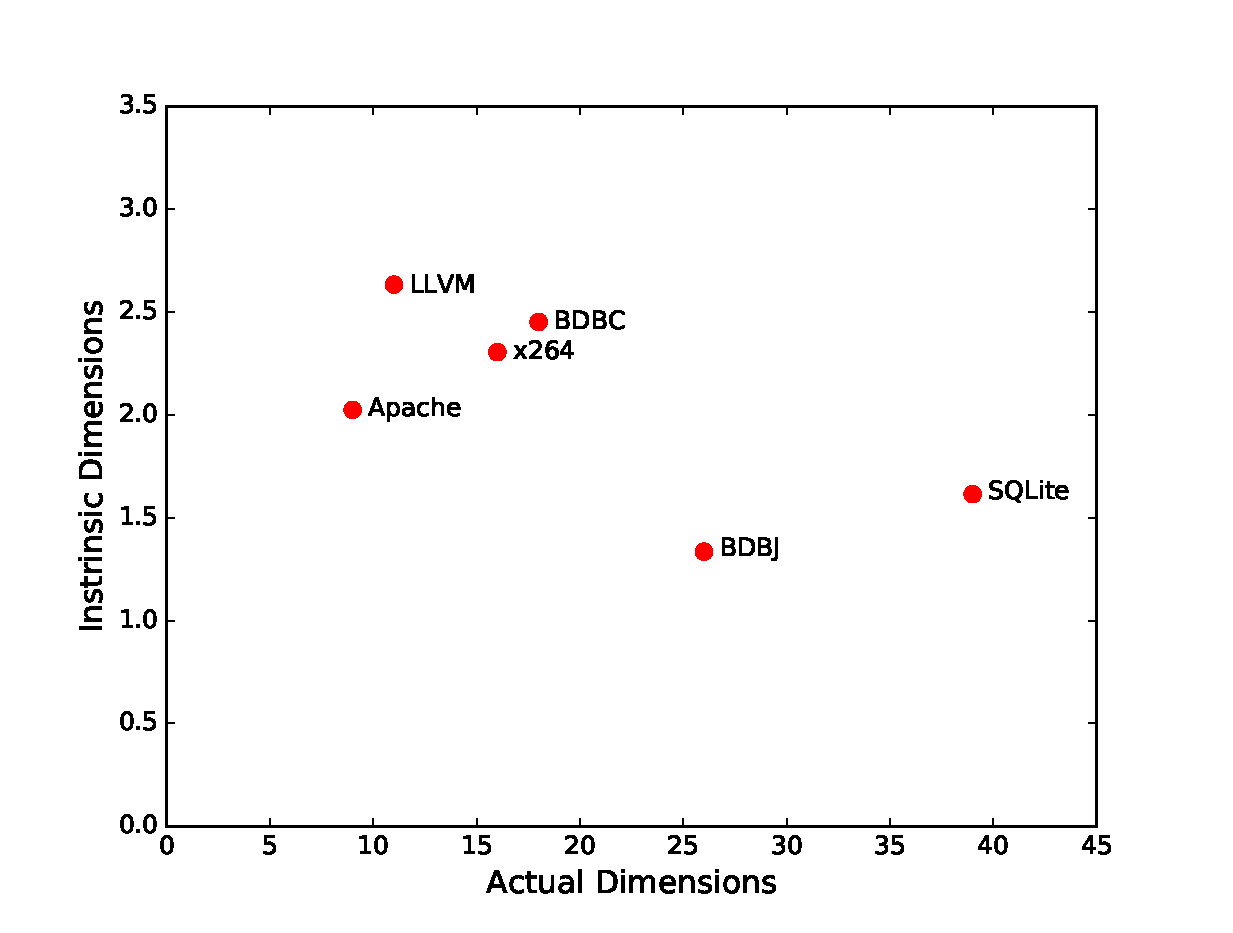
\includegraphics[width=0.9\columnwidth]{Figures/underlying_dimension}
\caption{Intrinsic dimensionality of the subjects systems are shown on the y-axis. The number on the side is the actual dimension of the system. The intrinsic dimensionality of the systems are much lower than the actual dimensionality (number of columns in the dataset).}
\label{fig:underlying_d}
\end{figure}
We observe that \textbf{the intrinsic dimensionality of the software system is much lower than the actual dimension}. Figure \ref{fig:underlying_d} presents the intrinsic dimensionality along with the actual dimensions of the software systems. If we take a look at the intrinsic dimensionality and compare it with the actual dimensionality, then it becomes apparent that the configuration space lies on a lower dimensional hyperplane. For example, SQLite has 39 configuration options but the intrinsic dimensionality of the space is just 7.61 (this is a fractal dimension). At the heart of \what is WHERE (a spectral clusterer), which uses the approximation of the first principal component to divide the configuration space and hence can take advantage of the low intrinsic dimensionality. 

As a summary, our observations indicates that the intrinsic dimension of the configuration space is much lower that its actual dimension. Hence, clustering based on the intrinsic dimensions rather than the actual dimension would be more effective. In other words, configurations with similar performance values lie closer in the intrinsic hyperplane when compared to the actual dimensions and may be the reason as to why \what achieves empirically good results.

\begin{myshadowbox}
The intrinsic dimension of the configuration space is much lower than its actual dimension and hence clustering based on the intrinsic dimension is more effective.
\end{myshadowbox}

\section{Reliability and Validity}\label{sect:construct}

{\em Reliability} refers to the consistency of the results obtained
from the research.  For example,   how well independent researchers
could reproduce the study? To increase external
reliability, this paper has taken care to either  clearly define our
algorithms or use implementations from the public domain
(SciKitLearn)~\cite{scikit-learn}. Also, all the data used in this work is available
on-line in the PROMISE code repository and all our algorithms
are on-line at github.com/ai-se/where.

{\em Validity} refers to the extent to which a piece of research actually
investigates what the researcher purports to investigate~\cite{SSA15}.
{\em Internal validity} checks if the differences found in
the treatments can be ascribed to the treatments under study. 

One internal validity issue with our experiments is the choice
of {\em training and testing} data sets discussed in 
\fig{systems}. Recall that while all our learners used the same
{\em testing} data set, our untuned learners were only given
access to {\em training} data.

Another internal validity issues is {\em instrumentation}. The very low $\mu$ and $\sigma$ error values
reported in this study are so small that it is reasonable to ask whether they are due to some instrumentation
quirk, rather than due to using a clever sample strategy:
\begin{itemize}
\item
Our low $\mu$ values are consistent with prior work (e.g.~\cite{sarkar2015cost});
\item
As to our low $\sigma$ values, we note that, when the  error values are so close to 0\,\%, the standard
deviation of the error is ``squeezed'' between zero and those errors. Hence, we would expect that
experimental rigs
that generate error values on the order of 5\,\% and \eq{err} should have $\sigma$ values of $0\le \sigma \le 5$ (e.g., like those seen in our introduction).
\end{itemize}

Regarding SQLite, we cannot measure all possible configurations in reasonable time. Hence, we sampled only 100 configurations to compare prediction and actual performance values. We are aware that this evaluation leaves room for outliers.
Also, we are aware that measurement bias can cause false interpretations~\cite{me12d}. Since we aim at predicting performance for a special workload, we do not have to vary benchmarks.



  We aimed at increasing the {\em external validity} by choosing software systems from different domains with different configuration mechanisms and implemented with different programming languages. Furthermore, the systems used are deployed and used in the real world. Nevertheless, assuming the evaluations to be automatically transferable  to all configurable software systems is not fair. To further strengthen external validity, we run the model (generated by \textit{\what + $S_1$}) against other optimizers, such as NSGA-II and differential evolution~\cite{storn1997differential}. That is, we validated whether the learned models are not only applicable for GALE style of perturbation. In Table~\ref{fig:external_validity}, we see that the models developed are valid for all optimizers, as all optimizers are able to find the near optimal solutions.



\section{Related Work}
\label{sect:related}
 
In 2000, Shi and Maik~\cite{shi00} claimed the term ``spectral clustering'' as a reference to their normalized cuts
image
segmentation algorithm that  partitions data through a spectral (eigenvalue) analysis of the  
Laplacian representation of the similarity graph between instances in the data.

In 2003, Kamvar et al.~\cite{kamvar2003spectral}  generalized that definition saying that ``spectral learners''
were any data-mining algorithm that first replaced the raw
dimensions with those inferred from the spectrum (eigenvalues) of the affinity (a.k.a.\ distance)
matrix of the data, optionally adjusted via some normalization technique).

Our clustering based on first principal component splits the data on a   approximation to an eigenvector, found at each recursive level
of the data (as described in \tion{spect}). 
Hence, this  method is a ``spectral clusterer'' in the general Kamvar sense. 
Note that,
for our data, we have
not found that Kamvar's normalization matrices are needed.

Regarding sampling, there are a wide range of methods know as experimental designs or designs of experiments~\cite{pukelsheim2006optimal}. They usually rely on fractional factorial designs as in the combinatorial testing community~\cite{Kuhn:2013}. 

Furthermore, there is a recent approach that learns {\em per\-for\-mance-influence models} for configurable software systems~\cite{SGA+15}. While this approach can handle even numeric features, it has similar sampling techniques for the Boolean features as reported in their earlier work~\cite{siegmund2012predicting}. Since we already compared to that earlier work and do not consider also numeric features, we did not compare our work to performance-influence models.
% (but perhaps if we were text mining
%on very large dimensional data, we would add in that normalization). 
 



\section{Conclusions}

Configurable software systems today are widely used in practice, but expose challenges
regarding finding performance-optimal configurations. State-of-the-art approaches require too
many measurements or are prone to large variances in their performance predictions. To avoid
these shortcomings, we have proposed a fast spectral learner, called \what,  along with three
new sampling techniques. The key idea of \what is to explore the configuration space with
eigenvalues of the features used in a configuration to determine exactly those configurations
for measurement that reveal key performance characteristics. 
This way, we can study many closely associated configurations with only a few measurements.

We evaluated our approach on six real-world configurable software systems borrowed from the
literature. Our approach achieves similar to lower error rates, while being stable when
compared to the state of the art. In particular, with the exception of Berkeley DB, our
approach is more accurate than the state-of-the-art approaches by Siegmund et
al.~\cite{siegmund2012predicting} and Guo et al.~\cite{guo2013variability}. Furthermore, we
achieve a similar prediction accuracy and stability as the approach by Sarkar et
al~\cite{sarkar2015cost}, while requiring a far smaller number of configurations to be
measured. We also demonstrated that our approach can be used to build cheap and stable
surrogate prediction models, which can be used by off-the-shelf optimizers to find the
performance-optimal configuration. 


